
In Part \ref{part:QGscale} of this thesis we have described in detail some particular energy scale, namely the species scale $\LSP$, which is gravitational in origin and moreover depends crucially on the light spectrum of the theory under consideration. Furthermore, the existence of such energy cut-off introduces important conceptual differences which strongly modify both semi-classical black hole physics as well as low energy effective field theory (EFT) considerations. In particular, since $\LSP$ can become arbitrarily smaller than the Planck scale in the presence of a large number of light species, it offers interesting resolutions to old theoretical problems (like the species problem, see Section \ref{s:speciesmotivation}), and even potential phenomenological explanations for the appearance of certain hierarchies in the Standard Model of particle physics \cite{Dvali:2007hz,Dvali:2007iv, Castellano:2023qhp}. On the other hand, from a more modern perspective, this energy scale becomes also interesting in relation with the Swampland program, since it links two key ingredients together in a rather direct way: The quantum gravity cut-off and the number of light degrees of freedom in our theories. Indeed, many of the most interesting quantum gravity conjectures that have been proposed and thoroughly tested in the literature --- using mostly string theory constructions and holography, such as the Distance conjecture \cite{Ooguri:2006in} or (the tower versions of) the Weak Gravity conjecture \cite{Arkani-Hamed:2006emk,Heidenreich:2016aqi,Andriolo:2018lvp,Montero:2016tif}, require from the existence of infinite towers of particle states that become light in Planck units when approaching certain limiting regimes within the gravitational EFT. Therefore, it is important to pinpoint what is the precise role that this energy cut-off plays within quantum gravity in general and, more specifically, in connection with the Swampland conjectures.

Regarding this important question, in Chapter \ref{ch:SpeciesIntro} we elaborated on how the identification of the maximum cut-off energy for any effective field theory weakly coupled to Einstein gravity with the species scale allows us to understand all these matters within the same theoretical framework. This means, in particular, that when writing any EFT expansion for gravity, the scale suppressing generic higher-curvature corrections should be given precisely by $\LSP$, such that one would expect to find the following expression in $d$ spacetime dimensions
%
\beq
\mathcal{L}_{\mathrm{EFT}}\, \supset\, \sqrt{-g} \left[\frac{1}{2 \kappa_d^2} \left(\mathcal{R} + \sum_{n >2} \frac{\mathsf{O}_n (\mathcal{R})}{\LSP^{n-2}}\right) -\frac{1}{2} G_{ij} (\phi) \partial_{\mu} \phi^i \partial^{\mu} \phi^j \right]\, ,
\label{eq:scalargravDlag}
\eeq
%
where as usual $\kappa_d^{2} =\Mpd^{2-d}$ controls the gravitational coupling constant, $\mathsf{O}_n (\mathcal{R})$ denotes any dimension-$n$ local operator involving higher powers of curvature invariants, and we have also included explicitly the kinetic terms for potentially massless/light scalar fields that may be present in the theory. Notice that this implies that the energy suppression of the aforementioned higher-dimensional operators can be smaller than naively expected, since depending on the vacuum we expand our theory around, $\LSP$ might be well below the Planck scale, thus providing for some gravitational `enhancement' of the Wilson coefficients associated to the set $\{ \mathsf{O}_n (\mathcal{R})\}$. In addition, one can argue that such UV cut-off \emph{must} depend non-trivially on the parameters defining the low energy EFT, which are typically controlled by the v.e.v.s of the light scalar fields $\phi^i$ in eq. \eqref{eq:scalargravDlag} above. This follows from the no-global symmetry conjecture (see Section \ref{s:SwamplandProgram} for details), since the existence of an absolute energy scale $\LSP$ in Planck units would imply the presence of some constant and physical parameter that cannot change dynamically in the theory, to which we can therefore associate an exact $(-1)$-form global symmetry. Hence, a more accurate statement would be that there exists some QG cut-off that generically varies over the moduli space of the theory, i.e. $\LSP= \LSP (\phi^i)$, which is indeed in agreement with general Swampland expectations, given that it is precisely when we probe some infinite distance limit in field space that we see a significant decrease in the quantum gravity scale.

Accordingly, our aim in this chapter we will to test this idea further using specific string theory constructions as a quantum gravity laboratory. Furthermore, given that this requires us to know the exact moduli dependence of the higher-curvature corrections under consideration, the strategy that we adopt will consist in focusing on those operators which are somehow protected, so that we can be sure that we are not missing any important information. This means, in practice, that we will restrict ourselves to analyze BPS operators in highly supersymmetric theories, for which the exact moduli dependence is known. Note that, strictly speaking, by doing so one cannot be entirely sure that the resulting behaviour indeed captures the scale we seek for, since there could be strong cancellations depending on the model we consider that would prevent us from extracting the relevant physics. Consequently, one should be careful to claim as general any quantitative information obtained from just observing a few low-lying higher-dimensional operators, but rather consider them to provide at least for some \emph{upper bound} on $\LSP$. %\AC{igual relacionar con BH entropy en Vafa Strominger. Similar caveats/considerations apply}

The chapter is hence organized as follows. In Section \ref{s:Exampleshighdim} we systematically analyze the moduli dependence of the first non-trivial higher-curvature corrections that have been already computed in the literature for all string theory constructions preserving 32 supercharges. More specifically, we consider ten-dimensional Type II string theories and toroidal compactifications thereof, with the relevant operators involving certain contractions of four Riemann tensors. In Section \ref{s:4dN=2} we consider instead theories preserving less amount of supersymmetry. Therefore, we focus mostly on Type II compactifications on Calabi--Yau three-folds, leading to 4d $\mathcal{N}=2$ supergravity EFTs, and study the moduli dependence of BPS operators involving fields only within the gravity multiplet. Finally, in Section \ref{s:summaryhigherops} we summarize our findings, putting special emphasis on the general lessons obtained and discussing certain important questions that our analysis raises as well as potentially interesting directions for future research. 

The material presented in this chapter is based on the publication \cite{Castellano:2023aum} adapted to better fit in the broader context of this thesis. (See also \cite{vandeHeisteeg:2023dlw} for a complementary viewpoint on these matters.)

\section{String theory examples in higher dimensions}
\label{s:Exampleshighdim}

In this section we restrict ourselves to maximally supersymmetric set-ups describing the low energy dynamics of certain string theory constructions in ten, nine and eight spacetime dimensions. The reason for doing so is that these theories are highly constrained (c.f. Section \ref{s:maxsugraintro}), which allows us to determine the moduli dependence of the Wilson coefficients associated to some higher-dimensional operators in an exact way. %The focus will be placed on whether these gravitational operators present a moduli dependent behaviour compatible with eq. \eqref{eq:gravEFTexpansion} above.

\subsection{ 10d Type IIB string theory}
\label{ss:10dIIB}

As our first example, we consider Type IIB string theory in ten dimensions, whose bosonic (two-derivative) pseudo-action in the Einstein frame is displayed by eq. \eqref{eq:IIB10d}. Moreover, as discussed in Section \ref{s:dualities}, this theory enjoys some non-perturbative $\mathsf{SL(2,\mathbb{Z})}$ duality symmetry, allowing us to arrange the supergravity fields into different representations of the duality group. In particular, the gravitational and scalar sectors of the theory can be written as follows 
%
\begin{equation}\label{eq:IIB10dSL2}
	S_\text{IIB}^{\text{10d}}\, \supset\, \frac{1}{2\kappa_{10}^2} \int \dd^{10}x\sqrt{-g} \left(\mathcal{R}-\frac{\partial \tau \cdot \partial \bar \tau}{2 (\text{Im}\, \tau)^2}\right)\, ,
\end{equation}
%
with $\tau=C_0 + \text{i} e^{-\phi}$ denoting the axio-dilaton. This pair of fields transform under $\mathsf{SL(2,\mathbb{Z})}$ as \cite{Schwarz:1995dk}
%
\begin{align}\label{eq:SdualitytransIIBdilaton}
	&\tau \rightarrow \frac{a\, \tau + b}{c\, \tau+d}\,,\qquad g_{\mu \nu} \rightarrow g_{\mu \nu}\, ,
\end{align}
%
where the constants $\{ a, b, c, d\}$ are integers satisfying $ad-bc=1$.

Crucially, since this theory has only one dimensionful parameter entering the supergravity action at the two-derivative level --- i.e. the Planck mass, we cannot obtain directly from it any useful information about the quantum gravity cut-off. To do this, what we should try instead is to look at higher-curvature operators which may be present in the theory, since those are expected to be suppressed by the quantum gravity scale.

Before doing so, let us take advantage from our knowledge acquired in precious chapters and try to guess how this function should look like. In particular, if the QG cut-off actually coincides with the species scale, one would expect it to be given by some sort of automorphic function\footnote{See Appendix \ref{ss:mathdefs} for the precise mathematical definition of an automorphic form.} that respects the duality symmetries of the theory. Furthermore, since at infinite distance the fundamental Type IIB string becomes weakly coupled, this function should behave asymptotically like the string scale. Our aim in the following will be to see whether or not these expectations are borne out in the present set-up.

\subsubsection*{The $\mathcal{R}^4$--\,operator}

Let us start by looking at the first non-trivial higher-curvature operator appearing in the 10d effective action. Such correction is $\frac12$-BPS protected, involves four powers of the Riemann tensor and has the following functional form \cite{Green:1999pv,Green:1997di,Pioline:1998mn}
%
\beq
S_\text{IIB}^{\text{10d}}\, \supset\, \frac{1}{\ell_{10}^2} \int \dd^{10}x \sqrt{-g}\, E_{3/2}^{sl_2} (\tau, \bar \tau)\, t_8 t_8 \mathcal{R}^4\, ,
\label{eq:10dR^4IIB}
\eeq
%
where $t_8 t_8 \mathcal{R}^4 \equiv t^{\mu_1 \ldots \mu_8} t_{\nu_1 \ldots \nu_8} \mathcal{R}^{\nu_1 \nu_2}_{\mu_1 \mu_2} \ldots \mathcal{R}^{\nu_7 \nu_8}_{\mu_7 \mu_8}$,\footnote{In fact, the actual term arising in the Type IIB effective action involves the $\mathcal{N}=(2,0)$ superinvariant $\mathcal{J}_0 = t_8 t_8 \mathcal{R}^4+ \frac{1}{8} \epsilon_{10}\epsilon_{10} \mathcal{R}^4$ \cite{Kiritsis:1997em}. Here $\epsilon_{10}$ denotes the Levi-civita tensor in ten dimensions and we have defined $\epsilon_{10}\epsilon_{10} \mathcal{R}^4 \equiv \epsilon^{\nu_1 \nu_2 \mu_1 \ldots \mu_8} \epsilon_{\nu_1 \nu_2 \rho_1 \ldots \rho_8} \mathcal{R}^{\rho_1 \rho_2}_{\mu_1 \mu_2} \ldots \mathcal{R}^{\rho_7 \rho_8}_{\mu_7 \mu_8}$.} and the tensor $t^{\mu_1 \ldots \mu_8}$ reads \cite{Green:1981ya}
%
\begin{equation}\label{eq:t8tensor}
\begin{aligned}
    t^{\mu_1 \ldots \mu_8} &= \frac{1}{5} \Big[ -2 \left( g^{\mu_1 \mu_3} g^{\mu_2 \mu_4} g^{\mu_5 \mu_7} g^{\mu_6 \mu_8} + g^{\mu_1 \mu_5} g^{\mu_2 \mu_6} g^{\mu_3 \mu_7} g^{\mu_4 \mu_8} + g^{\mu_1 \mu_7} g^{\mu_2 \mu_8} g^{\mu_3 \mu_5} g^{\mu_4 \mu_6}\right)\\
    & + 8 \left( g^{\mu_2 \mu_3} g^{\mu_4 \mu_5} g^{\mu_6 \mu_7} g^{\mu_1 \mu_8} + g^{\mu_2 \mu_5} g^{\mu_3 \mu_6} g^{\mu_4 \mu_7} g^{\mu_1 \mu_8} + g^{\mu_2 \mu_5} g^{\mu_6 \mu_7} g^{\mu_3 \mu_8} g^{\mu_1 \mu_4}\right)\\
    & - \left(\mu_1 \leftrightarrow \mu_2 \right) - \left(\mu_3 \leftrightarrow \mu_4 \right) - \left(\mu_5 \leftrightarrow \mu_6 \right) - \left(\mu_7 \leftrightarrow \mu_8 \right) \Big]\, .
\end{aligned}
\end{equation}
%
On the other hand, the quantity $E_{3/2}^{sl_2} (\tau, \bar \tau)$ appearing in \eqref{eq:10dR^4IIB} denotes the order--$\frac32$ non-holomorphic Eisenstein series of $\mathsf{SL(2,\mathbb{Z})}$, which is an automorphic form that can be defined as a series expansion in the complex valued field $\tau$ as follows (see Appendix \ref{ap:Massform} for details)
%
\begin{align}\label{eq:nonpertexpansionE3/2}
	E_{3/2}^{sl_2} =\, 2\zeta(3) \tau_2^{3/2} + 4\zeta(2) \tau_2^{-1/2} + \mathcal{O} \left( e^{-2\pi \tau_2}\right)\, .
\end{align}
%
Due to automorphicity, i.e. the fact that it remains invariant under the transformations \eqref{eq:SdualitytransIIBdilaton}, it is actually enough to restrict ourselves to the fundamental domain $\mathscr{F}$ of $\mathsf{SL(2,\mathbb{Z})}$ when studying e.g., the asymptotic behaviour of the function \eqref{eq:nonpertexpansionE3/2}. This leaves us with only one possible infinite distance limit to analyze, namely the weak coupling point $\tau_2 \to \infty$. Hence, at leading order, the $\mathcal{R}^4$--\,correction behaves like $\tau_2^{3/2}$ for large $\tau_2$. Now, since this operator has mass dimension $n=8$, eq. \eqref{eq:scalargravDlag} implies that its associated (generalized) Wilson coefficient should grow like $\left(\frac{\Mpt}{\LSP}\right)^{6}$. Therefore, given that the species scale coincides in the present case with the string scale asymptotically
%
\beq\label{eq:stringscale}
m_s=\frac{\Mpt}{\left(4\pi \tau_2^{2}\right)^{1/8}} \, ,
\eeq
%
we conclude that $\LSP^{-6} \sim \Mpt^{-6}\, \tau_2^{3/2}$, in agreement with the leading-order term in \eqref{eq:nonpertexpansionE3/2}. 

More generally, one can rewrite --- after Poisson resummation --- the series expansion \eqref{eq:nonpertexpansionE3/2}  in the following compact form (c.f. eq. \eqref{eq:nonholoEisenstein})
%
\beq\label{eq:E3/2Poisson}
E_{3/2}^{sl_2}(\tau, \bar \tau) = \sideset{}{'}\sum_{(p, q) \in \mathbb{Z}^2 }\frac{\tau_2^{3/2}}{\left| p+q\tau\right|^{3}}\, ,
\eeq
%
where the prime in the sum indicates that we should exclude the point $(0,0)$. Crucially, we can recognize the above expression as a  formal sum over all relevant $(p,q)$-string tensions 
%
\beq
E_{3/2}^{sl_2}(\tau, \bar \tau) = \left(4 \pi^{\frac34}\right)^3 \sideset{}{'}\sum_{(p, q) \in \mathbb{Z}^2 } \left( \frac{\Mpt}{\sqrt{T_{p,q}}}\right)^6\, , \qquad \text{with}\ \ T_{p,q}= \frac{2\pi}{\ell_{10}^2} \frac{\left| p+q\tau\right|}{\sqrt{\tau_2}}\, ,
\eeq
%
which indeed provide for the leading tower of states upon exploring other infinite distance points outside the fundamental domain $\mathscr{F}$, and hence determine the species scale asymptotically.

\subsubsection*{Further quantitative tests}

Additionally, one can try to extend the previous analysis by looking at the next few contributions to the four-(super)graviton effective action in 10d Type IIB string theory. These terms --- which still preserve some reduced amount of supersymmetry --- involve respectively four and six derivatives of $\mathcal{R}^4$ and they receive both perturbative and non-perturbative corrections. The first one, which corresponds to a gravitational operator of mass dimension $n=12$, can be computed to be \cite{Green:1999pu}
%
\beq
S_\text{IIB}^{\text{10d}}\, \supset\, \frac{\ell_{10}^2}{2} \int \dd^{10}x \sqrt{-g}\,E_{5/2}^{sl_2} (\tau, \bar \tau)\, \partial^4 \mathcal{R}^4\, ,
\label{eq:10dpartial4R^4IIB}
\eeq
%
and its moduli dependence is captured this time by the order--$\frac52$ non-holomorphic Eisenstein series. As it was also the case for the $\mathcal{R}^4$--\,term before, in order to check whether the expected expansion \eqref{eq:scalargravDlag} holds for this case as well we only need to study the large $\tau_2$ behaviour. Upon doing so, one finds (c.f. eq. \eqref{eq:nonpertexpansion})
%
\beq
E_{5/2}^{sl_2} (\tau, \bar \tau) =  2\zeta(5) \tau_2^{5/2} + \frac{4\pi^4}{135} \tau_2^{-3/2} + \mathcal{O}(e^{-4\pi\tau_2})\, ,
\eeq
%
which to leading order agrees with $\left(\frac{\Mpt}{\LSP}\right)^{10}$, where $\LSP=m_s$.

On the other hand, the second operator involving six derivatives of the Riemann tensor reads as follows\cite{Green:2005ba,Green:2010wi,Green:2010kv}
%
\beq
S_\text{IIB}^{\text{10d}}\, \supset\, \ell_{10}^4 \int \dd^{10}x \sqrt{-g}\, \mathcal{E} (\tau, \bar \tau)\, \partial^6 \mathcal{R}^4\, .
\label{eq:10dpartial6R^4IIA}
\eeq
%
where $\mathcal{E} (\tau, \bar \tau)$ is some particular modular function not of the Eisenstein type. It can be nevertheless expanded around $\tau_2\to \infty$, yielding
%
\beq
\mathcal{E} (\tau, \bar \tau) = \frac{2\zeta(3)^2}{3} \tau_2^{3} + \frac{4}{3}\tau_2 + \frac{8\zeta(2)^2}{5}\tau_2^{-1} + \frac{4\zeta(6)}{27}\tau_2^{-3} + \mathcal{O}(e^{-4\pi\tau_2})\, ,
\eeq
%
where the first term corresponds to the tree-level contribution, whilst the remaining pieces --- except for the exponentially suppressed corrections --- include up to three-loop contributions in $g_s$ (see \cite{Green:2010wi} and references therein). Notice that, since the above operator has mass dimension $n=14$, one expects according to eq. \eqref{eq:scalargravDlag} a dependence of the form $\LSP^{-12}\, \partial^6 \mathcal{R}^4$ in Planck units, which indeed matches asymptotically with the species scale computation.

Beyond four-point graviton scattering one may also consider higher-dimensional operators mixing the gravitational field with the Ramond-Ramond $p$-forms. In particular, there is an infinite family of such terms in the 10d Type IIB effective action which are of the form $\mathcal{R}^4 |G_3|^{4g-4}$ (c.f. discussion after eq. \eqref{eq:IIB10dSL2intro} for a precise definition of $G_3$). Note that these operators can be alternatively expressed, upon compactification on any hyper-K\"ahler manifold, in terms of $\mathcal{N}=4$ topological string theory \cite{Berkovits:1994vy} (see also \cite{Ooguri:1995cp}).\footnote{A similar phenomenon happens in 4d $\mathcal{N}=2$ theories, where certain higher derivative F-terms can be computed exactly by the $\mathcal{N}=2$ topological string, see Section \ref{s:4dN=2} below.} Moreover, their precise moduli dependence has been conjectured to be \cite{Berkovits:1998ex}
%
\begin{equation}\label{eq:BerkovitsVafa}
	\begin{aligned}
		S_\text{IIB}^{\text{10d}}\, \supset\, & \int \dd^{10}x\sqrt{-g}\, \mathcal{R}^4 \sum_{g\geq1} \ell_{10}^{4g-6} \alpha_{g} \sum_{k=2-2g}^{2g-2} (-1)^k \tau_2^{-2g+2}G_3^{2g-2+k} \bar{G}_3^{2g-2-k}\\
            &\sum_{(m, n) \in \mathbb{Z}^2 \setminus \lbrace (0,0) \rbrace} \frac{\tau_2^{g+1/2}}{\left( m+n\tau\right)^{g+1/2+k} \left( m+n \bar \tau\right)^{g+1/2-k}}\, ,
	\end{aligned}
\end{equation}
%
where $\{\alpha_g\}$ denote some unknown normalization coefficients. Notice that for $k=0$, the operators reduce to $\mathcal{R}^4 \left|\tau_2^{-1/2} G_3 \right|^{4g-4}$, which are manifestly modular invariant, have mass dimension $n=4g+4$ and their accompanying coefficients become $E_{g + 1/2}^{sl_2} (\tau, \bar \tau)$. Therefore, at infinite distance, each of these higher-derivative terms behaves like $\tau_2^{g +1/2} \propto \left(m_s/\Mpt \right)^{-4g-2}$, in perfect agreement with eq. \eqref{eq:scalargravDlag}.

\subsubsection*{A closer look into the EFT expansion}

There are a couple of important lessons that one can extract already from this simple example. On the one hand, if we just restrict ourselves to the first non-trivial gravitational correction described in \eqref{eq:10dpartial4R^4IIB}, it is natural to propose the modular form
%
\beq\label{eq:speciesIIB}
\LSP = \left(E_{3/2}^{sl_2} (\tau, \bar \tau)\right)^{-1/6}\, ,
\eeq
%
as being the perfect candidate for a species scale function globally defined over the entire 10d Type IIB moduli space. Furthermore, the function \eqref{eq:speciesIIB} satisfies the two minimal requirements that any bona-fide species scale must fulfill in the present case:
%
\begin{itemize}
    \item[$\circ$] $\LSP$ is bounded from above (since it cannot exceed $\Mpd$) and it vanishes asymptotically at infinite distance, namely $\LSP (\tau, \bar \tau) \to 0$ as $\tau \to \text{i} \infty$.

    \item[$\circ$] It is given by some \emph{automorphic} form, namely a modular invariant function of $\tau$ satisfying
%
\beq
 \notag \LSP \left(\frac{a \tau +b}{c\tau +d}\, , \, \frac{a \bar \tau +b}{c \bar \tau +d} \right) = \LSP (\tau, \bar \tau)\, , \qquad ad-cd=1\, ,
\eeq
%
where $a,b,c,d \in \mathbb{Z}$.
\end{itemize}
%
However, once we go beyond and consider additional higher-curvature corrections, we readily realize that they do not strictly organize in powers of the \emph{same} cut-off function, as the naive expectation from \eqref{eq:scalargravDlag} would suggest. Indeed, these moduli-dependent coefficients are seen to be given by certain automorphic forms of $\mathsf{SL(2,\mathbb{Z})}$, which nonetheless cannot be written as powers of one another. This precludes a priori from a canonical identification of the species scale function as any one of the aforementioned generalized Wilson coefficients. In any event, what remains undoubtedly true is that the gravitational EFT expansion proposed in eq. \eqref{eq:scalargravDlag} emerges when approaching any infinite distance point in the present 10d example. This is of course in agreement with our quantum field theory experience, since it is there where the weak coupling behaviour is usually restored \cite{Gendler:2020dfp}, and the classical dimensions of the different gravitational operators are actually reliable. On the contrary, when venturing towards the bulk of the moduli space, further perturbative and non-perturbative corrections may become important and thus significantly change the expectations from \eqref{eq:scalargravDlag}, which can be thought of as some sort of `anomalous dimensions'.

On the other hand, it should be mentioned that despite these difficulties for selecting any canonical representative for $\LSP (\tau, \bar \tau)$, certain qualitative features such as the presence and location of a \emph{desert point} \cite{Long:2021jlv, vandeHeisteeg:2022btw} --- i.e. the locus where the quantum gravity cut-off is maximized, do not crucially depend on which operator one chooses to focus on. In particular, all these modular forms present an absolute minimum at the cusp $\tau= e^{\frac{2\pi \text{i}}{3}}$, thus coinciding with the point where the the BPS gap of $(p,q)$-strings is maximized (c.f. eq. \eqref{eq:E3/2Poisson}).


\subsection{ 10d Type IIA string theory}
\label{ss:10dIIA}

We now turn to ten-dimensional Type IIA string theory, whose bosonic action can be found in eq. \eqref{eq:IIA10dEinsteinframeaction}. This theory has simpler moduli space than its Type IIB counterpart, which it is actually isomorphic to the real line when parametrized in terms of the dilaton v.e.v. $\braket{\phi}$. Relatedly, the Type IIA theory does not enjoy any non-trivial U-duality properties, preventing us from inferring a priori which kind of functions should appear in the gravitational EFT expansion. In any event, we can still consider the first few non-zero corrections to the supergravity action and explicitly analyze its moduli dependence. The first one of these happens to be protected again by supersymmetry, and it reads as follows \cite{Grisaru:1986dk,Grisaru:1986kw,Gross:1986iv} 
%
\beq
S_\text{IIA}^{\text{10d}}\, \supset\, \frac{1}{\ell_{10}^2} \int \dd^{10}x \sqrt{-g}\, \left( 2\zeta(3) e^{-3\phi/2} + \frac{2\pi^2}{3} e^{\phi/2}\right) t_8 t_8 \mathcal{R}^4\, ,
\label{eq:10dR^4IIA}
\eeq
%
which is nothing but the expression \eqref{eq:10dR^4IIB} with the instanton sum excluded. In fact, the first term corresponds to the tree-level contribution (which arises at fourth-loop order in the 2d sigma-model perturbation theory), whilst the second piece is a one-loop correction in $g_s$. 

Let us now check what are the relevant asymptotics of this dimension-8 operator. At weak coupling, namely when $\phi \to -\infty$ (equivalently $g_s \to 0$), the tree-level term dominates and we obtain
%
\beq
\mathcal{L}_{\mathcal{R}^4}^{\text{10d}}\, \sim\, \sqrt{-g} \left(\frac{2\zeta(3)}{\ell_{10}^2} e^{-3\phi/2} \right) t_8 t_8 \mathcal{R}^4\ .
\label{eq:R^4weakcoupling}
\eeq
%
Comparing this with eq. \eqref{eq:scalargravDlag}, we deduce that the coefficient accompanying such coupling in the effective action should behave like $\left(\frac{\Mpt}{\LSP}\right)^{6}$ asymptotically. Therefore, since the species scale coincides with the string scale along the weak coupling limit, we again find that
%
\beq
\left(\frac{\Mpt}{\LSP}\right)^{6}\, =\, (4\pi)^{3/4}e^{-3\phi/2}\, ,
\eeq
%
in agreement with eq. \eqref{eq:R^4weakcoupling} above.

On the contrary, at strong coupling, it is the one-loop correction which becomes more important, thus leading to the following asymptotic dilaton dependence
%
\beq
\mathcal{L}_{\mathcal{R}^4}^{\text{10d}}\, \sim\, \sqrt{-g} \left(\frac{4\zeta(2)}{\ell_{10}^2} e^{\phi/2} \right) t_8 t_8 \mathcal{R}^4 \ .
\label{eq:R^4strongcoupling}
\eeq
%
Crucially, the species counting is now dominated by the tower of D0-brane bound states instead, since the fundamental string becomes infinitely heavy in 10d Planck units. Following the original definition of $\LSP$ in \eqref{species}, one recovers that the species scale is capturing the 11d M-theory Planck mass, which is given by
%
\beq \label{eq:QGscaleandN} 
		\LSP\, \sim\, m_{\text{D}0}^{1/9}\ \Mpt^{8/9}\, \sim\,  e^{-\phi/12} \Mpt\, ,
\eeq
%
such that the quantity $\LSP^{-6}\, \mathcal{R}^4$ precisely reproduces the leading-order piece \eqref{eq:R^4strongcoupling}. Note that the previous conclusion strongly rests on the fact that there are no further loop corrections to $t_8 t_8 \mathcal{R}^4$ in Type IIA string theory, since otherwise the matching with the 11d Planck scale would be automatically spoiled. 

Finally, let us comment that by performing a similar analysis to the one done for the 10d Type IIB theory regarding the corrections of the form $\partial^4 \mathcal{R}^4$ and $\partial^6 \mathcal{R}^4$, it can be readily seen that they are in fact not suppressed by the species scale to the expected power when the M-theory limit is probed. In contrast, it is the mass scale of the lightest tower (i.e. the D0-branes) the one controlling the suppression. For emergent string limits, however, we still find that they always appear with the correct power of $\LSP$, but one must take into account that in such cases the species scale and that of the tower coincide, namely $\LSP = m_s$. We elaborate further on this point in Section \ref{ss:gravEFTexpansion} below.

\subsection{M-theory on $\mathbf{T}^2$}
\label{ss:MthyT2}

Let us now turn to the unique 9d $\mathcal{N}=2$ supergravity theory, which may be obtained by e.g., compactifying M-theory on a $\mathbf{T}^2$ with an internal metric of the form
%
\begin{equation}\label{eq:T2metric}
	g_{m n}= \frac{\mathcal{V}_2}{\tau_2} \left(
	\begin{array}{cc}
		1 & \tau_1  \\
		\tau_1 & |\tau|^2  \\
	\end{array}
	\right) \, ,
\end{equation}
%
where $\tau=\tau_1+{\rm i}\tau_2$ denotes the complex structure of the torus and $\mathcal{V}_2$ its overall volume. The scalar and gravitational sectors in the 9d Einstein frame read (see Section \ref{ss:9dmaxsugra} for details)
%
\begin{equation}\label{eq:9dchap5}
	S_\text{M-th}^{\text{9d}} \supset \frac{1}{2\kappa_9^2} \int \dd^{9}x\, \sqrt{-g}\,  \left[ \mathcal{R} - \frac{9}{14} \frac{\left( \partial \mathcal{V}_2 \right)^2}{\mathcal{V}_2^2} -\frac{\partial \tau \cdot \partial \bar \tau}{2 \tau_2^2} \right]\, ,
\end{equation}
%
therefore exhibiting some non-trivial moduli space which is moreover classically exact and parametrizes the manifold $\mathcal{M}_{\text{9d}}=\mathsf{SL(2,\mathbb{Z})}\backslash \mathsf{SL(2,\mathbb{R})}/\mathsf{U(1)} \times \mathbb{R}_{+}$ (after quotient out the $\mathsf{SL(2,\mathbb{Z})}$ U-duality symmetry \cite{Schwarz:1995dk,Aspinwall:1995fw}). 

Our strategy here will again consist in studying the asymptotic moduli dependence featured by certain protected quantities in the low energy action, so as to see whether the expectations arising from the species counting are furnished in the present example as well. Hence, we look at the next non-trivial correction to the two-derivative lagrangian \eqref{eq:9dchap5}, which again behaves schematically like $\mathcal{R}^4$, and is still BPS protected. Its dependence with respect to the moduli space parametrized by $\lbrace \mathcal{V}_2, \tau \rbrace$ has been already computed in \cite{Green:1997tv,Green:1997as}, and is captured by the following non-trivial function (see also \cite{Green:2010wi})
%
\beq
S_\text{M-th}^{\text{9d}} \supset \frac{1}{\ell_{9}} \int \dd^{9}x \sqrt{-g}\, \left( \frac{2\pi^2}{3} \mathcal{V}_2^{6/7} + \mathcal{V}_2^{-9/14} E_{3/2}^{sl_2} (\tau, \bar \tau)\right) t_8 t_8 \mathcal{R}^4\, ,
\label{eq:9dR^4MthT2}
\eeq
%
where $\mathsf{SL(2,\mathbb{Z})}$ invariance is readily manifest (recall that the volume modulus is left unchanged under a modular transformation). The above operator has mass dimension $n=8$, such that the function in parenthesis is expected to behave like $\left(\frac{M_{\rm Pl;\, 9}}{\LSP}\right)^{6}$ at any infinite distance boundary of $\mathcal{M}_{\text{9d}}$. In the following, we consider each of these limits in turn (see Figure \ref{fig:MthyT2} below), with the important simplification that one can restrict to a subset of the latter for which $\tau_2 \to \infty$, thanks to $\mathsf{SL(2,\mathbb{Z})}$ invariance. Furthermore, we note that depending on whether $\tau_2 > \mathcal{V}_2$ or $\tau_2 < \mathcal{V}_2$, the second/first term in eq. \eqref{eq:9dR^4MthT2} dominates, which allows us to divide the fundamental domain of the phase diagram into two different subregions.
\newline

%%%%%%%%%%%
\begin{figure}[htb]
\begin{center}
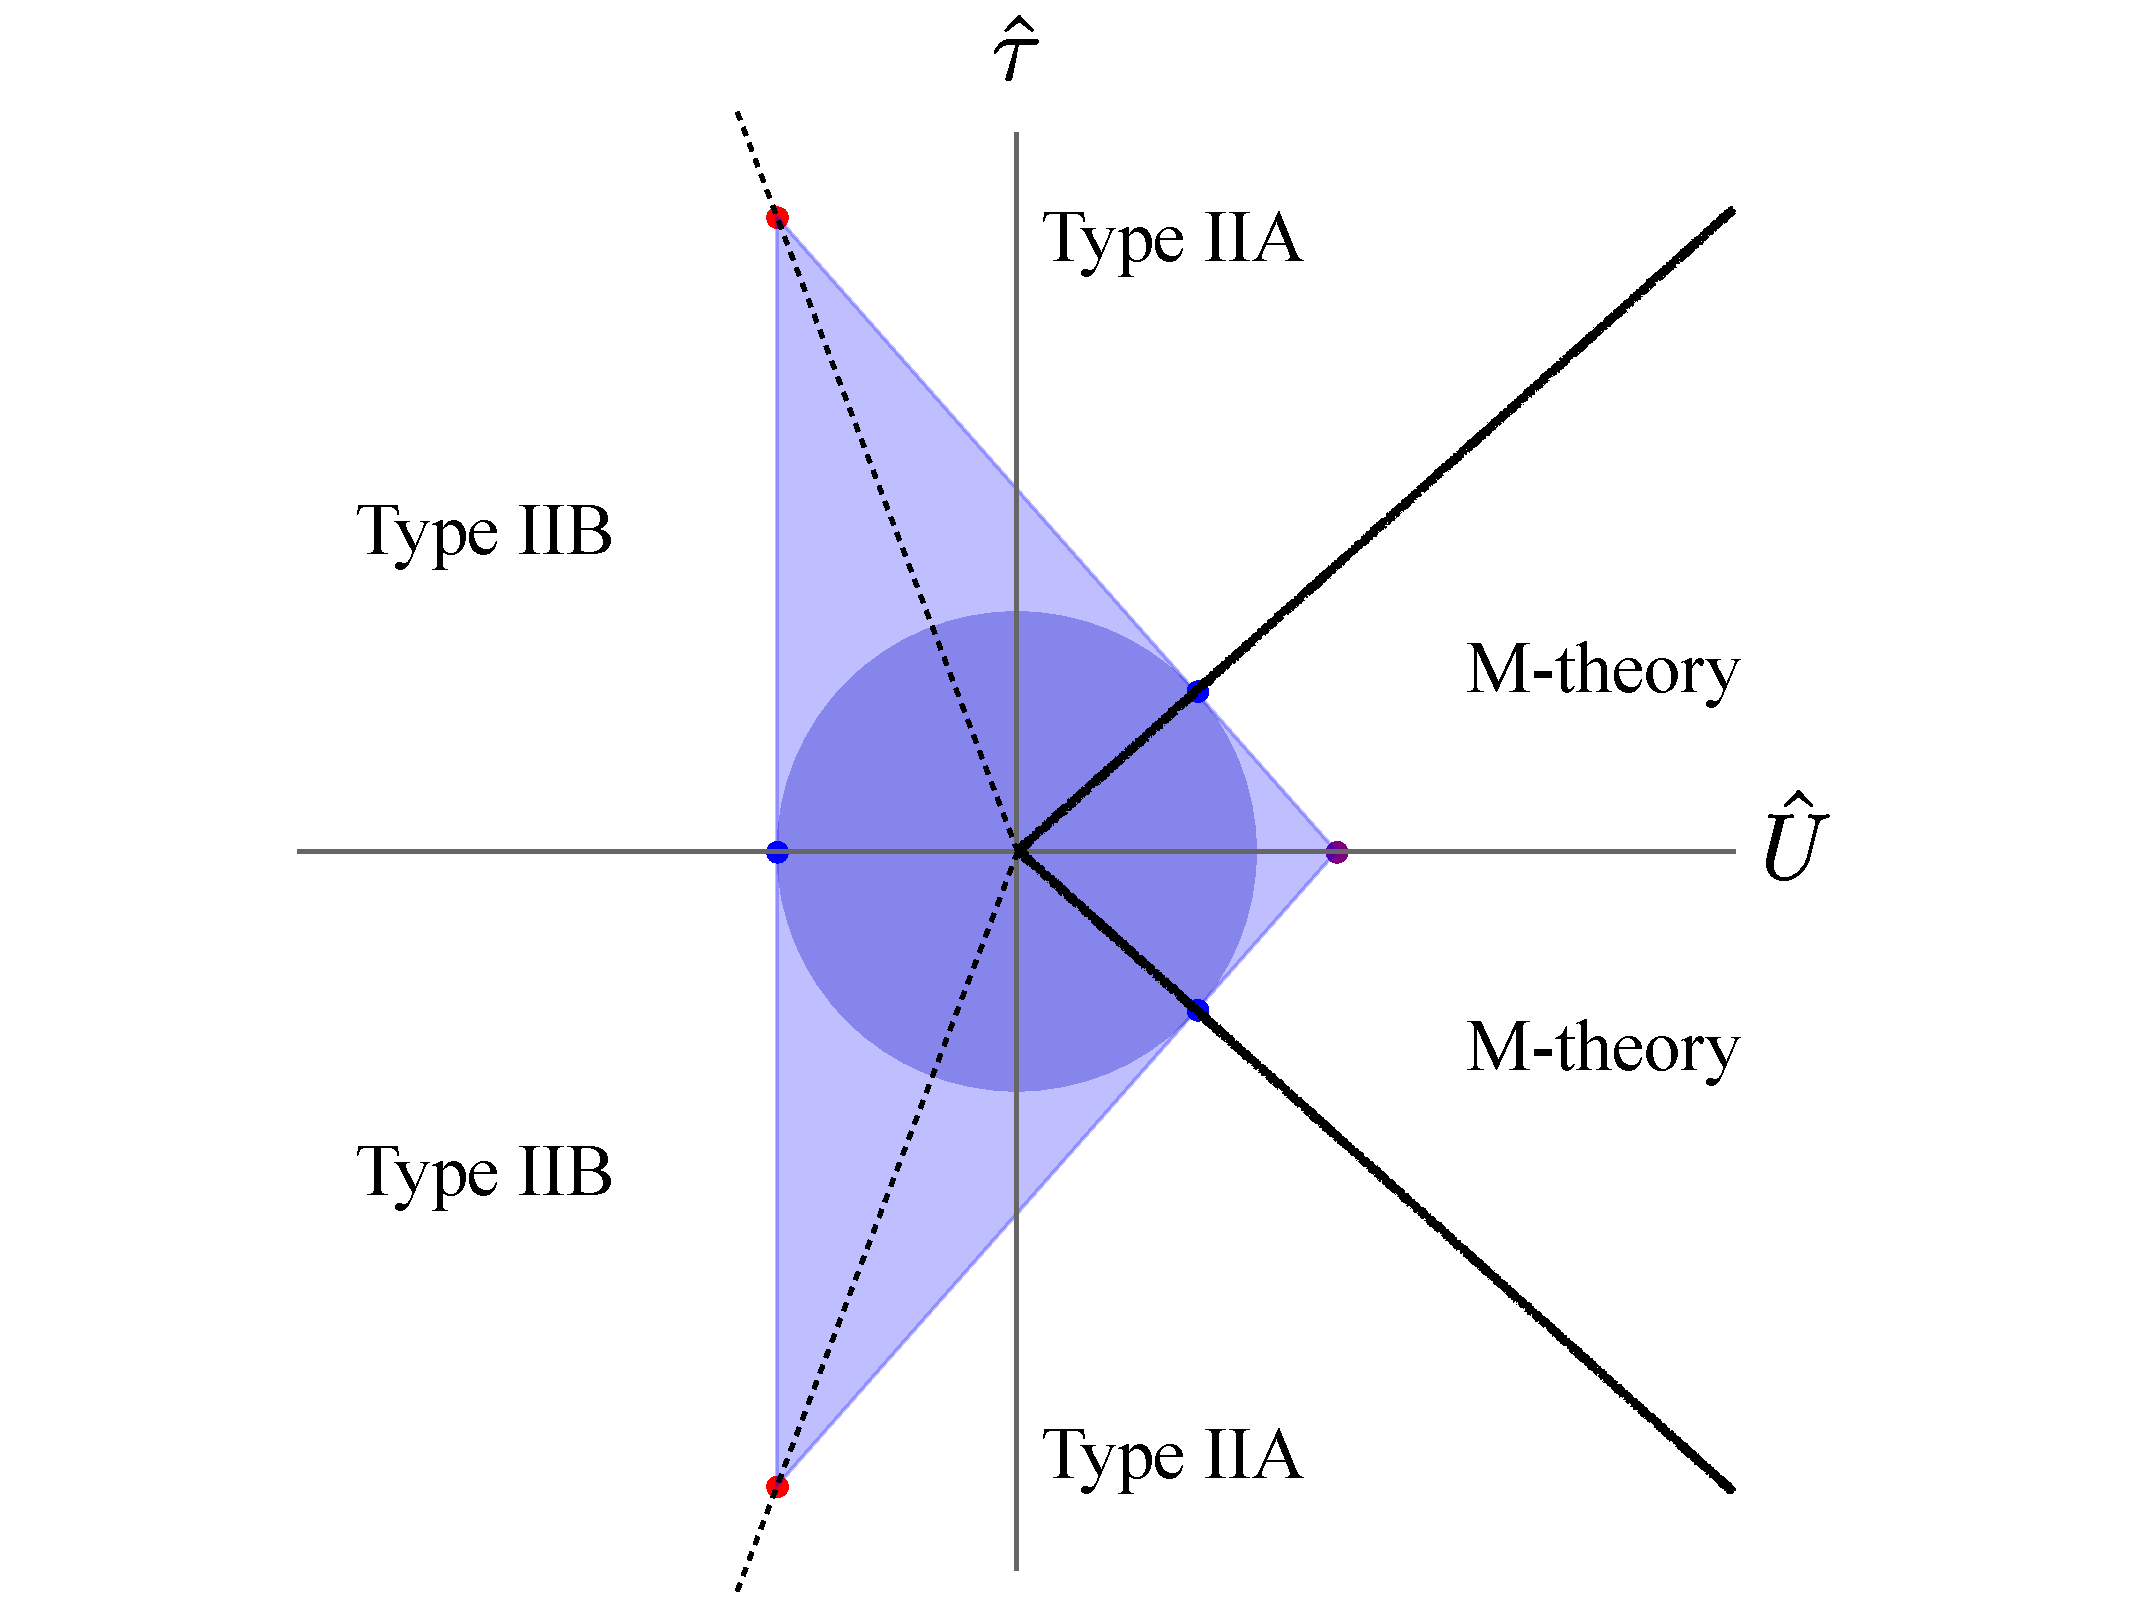
\includegraphics[width=0.6\textwidth]{CH-1-1v2.pdf}
\caption{\small Phase diagram for the (asymptotic) species scale in M-theory on $\mathbf{T}^2$, parametrized by the canonical variables $\{ \hat U = \frac{3}{\sqrt{14}} \log \mathcal{V}_2\, ,\, \hat \tau= \frac{1}{\sqrt{2}}\log \tau_2\}$. The blue dots are associated to circle decompactifications (possibly to a dual frame), whereas the red and purple ones signal emergent Type II string limits and full decompactification to eleven dimensions, respectively. The self-dual line $\hat{\tau}=0$ is fixed under the U-duality symmetry.}
\label{fig:MthyT2}
\end{center}
\end{figure}
%%%%%%%%%%%

\underline{\textit{The M-theory regime}}
\newline

Let us start with the region $\mathcal{V}_2 > \tau_2$. In this case, the dominant term in the expression for the $\mathcal{R}^4$--\,operator depends solely on the internal volume, so that one can restrict in practice to the large radius limit at fixed (and finite) complex structure. This is nothing but a full decompactification to 11d supergravity, and thus the species scale should coincide (up to order one factors) with the 11d Planck scale, which depends on the moduli fields as follows
%
\beq
\frac{M_{\rm Pl;\, 11}}{M_{\rm Pl;\, 9}}\, =\, (4\pi)^{-2/9}\, \mathcal{V}_2^{-1/7}\, .
\label{eq:11dPlanckmass}
\eeq
%
Therefore, according to eq. \eqref{eq:scalargravDlag} we expect the asymptotic behavior $\LSP^{-6} \sim \mathcal{V}_2^{6/7}$ arising in front of the quartic correction to the 9d action, which indeed matches the correct result. 
\newpage

\underline{\textit{The Type II regime}}
\newline

In the opposite regime, namely when $\tau_2 > \mathcal{V}_2$, the species scale should be controlled by the fundamental string mass (defined here as $m_{\text{str}} \equiv \sqrt{T_{\text{str}}}$), which corresponds to the red dot in the upper half-plane in Figure \ref{fig:MthyT2}. This can be readily computed, yielding
%
\beq
\frac{m_{\text{str}}}{M_{\rm Pl;\, 9}}\, =\, \frac{(4\pi)^{5/14}}{\sqrt{2}}\, \mathcal{V}_2^{3/28} \, \tau_2^{-1/4}\, .
\label{eq:fundstringmass9d}
\eeq
%
Hence, focusing in the second term in \eqref{eq:9dR^4MthT2} and using the asymptotic behaviour exhibited by the order--$\frac32$ non-holomorphic Eisenstein series (c.f. eq. \eqref{eq:nonpertexpansionE3/2}), we conclude that the coefficient of the $\mathcal{R}^4$--\,operator behaves asymptotically as $\mathcal{V}_2^{-9/14}\, \tau_2^{3/2} \sim m_{\text{str}}^{-6}$, in agreement with \eqref{eq:scalargravDlag}.
\newline

\underline{\textit{Decompactification to 10d}}
\newline

For completeness, let us also discuss the two boundaries between the different asymptotic regions in moduli space, as seen from the diagram in Figure \ref{fig:MthyT2}. These are moreover associated to certain asymptotic directions signalling towards partial decompactification to either 10d Type IIA or Type IIB string theory. On the one hand, precisely when $\tau_2 = \mathcal{V}_2 \to \infty$, a subset of KK modes become light and the theory decompactifies to 10d Type IIA supergravity. The 10d Planck scale presents the following moduli dependence
%
\beq
\frac{M^{\rm IIA}_{\rm Pl;\, 10}}{M_{\rm Pl;\, 9}}\, =\, (4\pi)^{1/56}\, \mathcal{V}_2^{-9/112} \tau_2^{-1/16} \sim \mathcal{V}_2^{-1/7}\, ,
\label{eq:10dPlanckmassIIA}
\eeq
%
which agrees asymptotically with both $M_{\rm Pl;\, 11}$ and $m_{\text{str}}$ along the aforementioned limit. Therefore, upon inserting $\LSP \sim M^{\rm IIA}_{\rm Pl;\, 10}$ into eq. \eqref{eq:scalargravDlag}, one reproduces the behaviour exhibited by \eqref{eq:9dR^4MthT2}.

On the other hand, for the limit $\mathcal{V}_2 \to 0$ the species counting is dominated by M2-branes wrapping the internal space. These states correspond to the KK tower implementing the M-theory/F-theory duality (see Section \ref{ss:dualitieswithlowersusy} for details), such that the quantum gravity scale becomes identical to the 10d Type IIB Planck mass, which reads
%
\beq
\frac{M^{\rm IIB}_{\rm Pl;\, 10}}{M_{\rm Pl;\, 9}}\, =\, (4\pi)^{1/56}\, \mathcal{V}_2^{3/28}\, .
\label{eq:10dPlanckmass}
\eeq
%
Hence, along such limit the $\mathcal{R}^4$--\,operator should be controlled by $\LSP^{-6} \sim \mathcal{V}_2^{-9/14}$, thus matching the behaviour observed in the second term of \eqref{eq:9dR^4MthT2}.

Before turning to higher-dimensional operators other than $t_8 t_8 \mathcal{R}^4$, let us make one more comment. Indeed, from the discussion above one would be tempted to propose $\LSP$ to be defined in the present nine-dimensional set-up precisely by
%
\beq
\LSP = \left( \frac{2\pi^2}{3} \mathcal{V}_2^{6/7} + \mathcal{V}_2^{-9/14} E_{3/2}^{sl_2} (\tau)\right)^{-1/6}\, ,
\label{eq:9dfullspeciesfn}
\eeq
%
which is automorphic and moreover reproduces the correct asymptotic behaviour in every infinite distance corner of $\mathcal{M}_{\text{9d}}$, as we just demonstrated. However, let us stress that this would imply, via eq. \eqref{eq:scalargravDlag}, that all subsequent higher order gravitational operators in the 9d effective action should also be accompanied by appropriate powers of the function \eqref{eq:9dfullspeciesfn}, which is known to be \emph{not} the case, see below. What seems to be true, though, is the fact that the species scale, as one typically defines it close to the infinite distance boundaries in moduli space (c.f. Section \ref{ss:Planck&string}), is the energy scale organizing the asymptotic EFT expansion of our quantum-gravitational theories, and thus should be taken as the true QG cut-off.  

%Second, notice that the function controlling the $t_8 t_8 \mathcal{R}^4$ interaction here is again an eigenfunction (with eigenvalue equal to $6/7$) of the Laplace operator in $SL(2,\mathbb{R})/SO(2) \times \mathbb{R}_+$
%
%\beq\label{eq:laplacian9d}
%\Delta_{\text{9d}} = \Delta_2 - \frac{7}{9}\, \mathcal{V}_2\, \partial_{\mathcal{V}_2} \left( \mathcal{V}_2\, \partial_{\mathcal{V}_2} \right) - \frac{1}{3}\, \mathcal{V}_2\, \partial_{\mathcal{V}_2}\, ,
%\eeq
%
%with $ \Delta_2 = \tau_2^2 \left( \partial^2_{\tau_1} + \partial^2_{\tau_2}\right)$. This was also the case in the 10d Type IIB case discussed before, and the eigenvalue seems to be related to the power of the number of species that accompanies the operator under consideration.
\subsubsection*{Further quantitative tests}

Proceeding as in the previous ten-dimensional examples, let us now look at the next few contributions to the four-(super)graviton effective action in 9d M-theory. For the four-derivative quartic term, the exact moduli dependence has already been obtained in the literature, leading to \cite{Green:2010wi}
%
\beq
S_\text{M-th}^{\text{9d}} \supset \ell_{9}^3 \int \dd^{9}x \sqrt{-g}\, \left( \frac{1}{2} \mathcal{V}_2^{-15/14} E_{5/2}^{sl_2} (\tau) + \frac{2\zeta(2)}{15} \mathcal{V}_2^{27/14} E_{3/2}^{sl_2} (\tau) + \frac{4\zeta(2)\zeta(3)}{15} \mathcal{V}_2^{-18/7}\right) \partial^4 \mathcal{R}^4\, .
\label{eq:9dpartial4R^4}
\eeq
%
Notice that such term is again compatible with $\mathsf{SL(2,\mathbb{Z})}$ invariance, so that we can restrict to the fundamental domain $\{ \tau \in \mathscr{F}\, ,\, \mathcal{V}_2 \geq 0\}$ in what follows. Moreover, the mass dimension of the $\partial^4 \mathcal{R}^4$--\,operator is $n=12$, such that according to \eqref{eq:scalargravDlag}, we expect an asymptotic dependence for the generalized Wilson coefficient of the form $\left(\frac{M_{\rm Pl;\, 9}}{\LSP}\right)^{10}$. Interestingly, this prediction is fulfilled in all the cases in which we probe an emergent string limit, namely when $\LSP = m_{\rm str}$, whereas in decompactification limits (either to ten or eleven dimensions) one cannot directly identify $\LSP^{-10}$ as the coefficient appearing in front of this operator. Still, this might be understood in terms of the dimensionality of the aforementioned operators, as we comment in Section \ref{ss:gravEFTexpansion} with more detail. %whereas for $t_8 t_8 R^4$ this is the case and we believe it to be the relevant term in the expansion for the identification of the species scale.


\subsection{M-theory on $\mathbf{T}^3$}
\label{ss:MthyT3}

As our final example, we consider maximal supergravity in eight spacetime dimensions. This theory arises upon compactifying e.g., Type IIB supergravity on a two-dimensional torus, leading to the following 8d action in the scalar-tensor sector
%
\begin{equation}\label{eq:IIB8d}
		\begin{aligned}
			S_\text{IIB}^{\text{8d}}\, \supset\, & \frac{1}{2\kappa_{8}^2} \int \dd^{8}x\sqrt{-g} \left[\mathcal{R}-\frac{1}{6}\frac{(\partial \nu)^2}{\nu^2} -\frac{\partial \tau \cdot \partial \bar \tau}{2 \tau_2^2} -\frac{\partial U \cdot \partial \bar U}{2 U_2^2} - \nu \frac{\left| \tau \partial b + \partial c\right|^2}{2\tau_2}\right]\, ,
		\end{aligned}
\end{equation}
%
where $U$ denotes the complex structure of the torus, $\nu= \left( \tau_2 V_2^2\right)^{-1}$ is an $\mathsf{SL(2,\mathbb{Z})}_{\tau}\,$--\, invariant volume, and $\{ b,c\}$ are compact scalar fields arising from the reduction of the NS and RR 2-form fields of 10d $\mathcal{N}=(2,0)$ supergravity along the internal 2-cycle. Note that there are two modular symmetries visible from the action \eqref{eq:IIB8d} above: that associated to the axio-dilaton --- which is inherited from ten dimensions, as well as an additional one which transforms the complex $U$ field in a fractional linear fashion. There is, however, an extra `hidden' $\mathsf{SL(2,\mathbb{Z})}_{T}$ symmetry associated to the K\"ahler modulus $T=b+ \i V_2$, %\footnote{Note that upon performing a T-duality on any of the two 1-cycles within the $\mathbf{T}^2$, one arrives at Type IIA string theory on a (dual) torus, which is moreover described by the same exact action as in eq. \eqref{eq:IIB8d} with the $U$ and $T$ fields exchanged.}
which can be made manifest upon changing variables from $\lbrace \nu, \tau\rbrace \leftrightarrow \lbrace \varphi_8, T\rbrace$ (c.f. eq. \eqref{eq:8dIIB}), where $\varphi_8$ denotes the 8d dilaton
%
\begin{equation}\label{eq:8ddilaton}
     e^{-2\varphi_8} = e^{-2\phi} V_2\, .
\end{equation}
%
What is important for us here is that the \emph{full} U-duality symmetry of the theory is actually larger, namely it consists of $\mathsf{SL(2,\mathbb{Z})} \times \mathsf{SL(3,\mathbb{Z})}$, where the modular factor acts solely on the complex structure modulus. In fact, upon introducing the following symmetric  $3\times3$ matrix with unit determinant \cite{Liu:1997mb}
%
\beq\label{eq:SL3matrix}
 \mathcal{B}= \nu^{1/3} \begin{pmatrix}
		\frac{1}{\tau_2} \quad  \frac{\tau_1}{\tau_2} \quad \frac{c+\tau_1 b}{\tau_2}\\ \frac{\tau_1}{\tau_2} \quad  \frac{|\tau|^2}{\tau_2} \quad \frac{\tau_1 c+|\tau|^2 b}{\tau_2}\\ \frac{c+\tau_1 b}{\tau_2} \quad  \frac{\tau_1 c+|\tau|^2 b}{\tau_2} \quad \frac{1}{\nu} + \frac{|c+\tau b|^2}{\tau_2}
	\end{pmatrix}\, ,
\eeq
%
which transforms in the adjoint representation of $\mathsf{SL(3,\mathbb{Z})}$, one can rewrite the above action in a manifestly $\mathsf{SL(2,\mathbb{Z})} \times \mathsf{SL(3,\mathbb{Z})}$ invariant way\footnote{Both $\mathsf{SL(2,\mathbb{Z})}_{\tau}$ and $\mathsf{SL(2,\mathbb{Z})}_{T}$ transformations are embedded within $\mathsf{SL(3,\mathbb{Z})}$ as upper and lower block-diagonal subgroups \cite{Kiritsis:1997em}.} 
%
\begin{equation}\label{eq:IIB8dSL3}
			\begin{aligned}
				S_\text{IIB}^{\text{8d}}\, \supset\, & \frac{1}{2\kappa_{8}^2} \int \dd^{8}x\sqrt{-g} \left[\mathcal{R} -\frac{\partial U \cdot \partial \bar U}{2 U_2^2} + \frac{1}{4} \text{tr} \left( \partial \mathcal{B} \cdot \partial \mathcal{B}^{-1} \right) \right]\, .
			\end{aligned}
\end{equation}
%
Therefore, we conclude that the moduli space of the theory is described by a group coset of the form $\mathcal{M}_{\text{8d}}=\mathsf{SL(2,\mathbb{Z})}\backslash \mathsf{SL(2,\mathbb{R})}/\mathsf{U(1)} \times \mathsf{SL(3,\mathbb{Z})}\backslash \mathsf{SL(3,\mathbb{R})}/\mathsf{SO(3)}$, where we have modded out by the U-duality group of the 8d theory.
	
In the following, it will be useful to phrase all our discussion using a dual description in terms of M-theory compactified on $\mathbf{T}^3$, whose bosonic action was already introduced in Section \ref{ss:8dmaxsugra}. Recall that the relevant scalar degrees of freedom, as seen from this dual perspective, are associated to the internal metric $g_{mn}$, the overall volume modulus $\mathcal{V}_3$ and a compact field $C^{(3)}_{123}$, which arises by reducing the antisymmetric 3-form field along the torus. In particular, one can make direct contact with the previous Type IIB description using a chain of dualities (see discussion around eqs. \eqref{eq:8dap} and \eqref{eq:8dIIA}), thus relating the complex structure modulus $U$ with some complex-valued field $\mathcal{T}$, namely
%
\beq\label{eq:T3complexvolume}
\mathcal{T}= C^{(3)}_{123}+ \text{i} \mathcal{V}_3\, ,
\eeq
%
as well as the matrix $\mathcal{B}$ in \eqref{eq:SL3matrix} with the \emph{unimodular} metric components of the compact space, i.e. $\tilde{g}_{m n}= \mathcal{V}_3^{-2/3} g_{mn}$. This recovers the action \eqref{eq:8dsl3} written in a manifestly $\mathsf{SL(3,\mathbb{Z})}$ invariant form. Furthermore, we will choose a parametrization of the scalar manifold that breaks the underlying duality symmetry of the theory, since it is better adapted for the discussion that is to follow as well as for the rest of the thesis. This amounts to selecting some $\mathbf{T}^2$ within the $\mathbf{T}^3$, compactify the 11d theory on it, and subsequently reduce the 9d supergravity EFT on an extra $\mathbf{S}^1$, thus leading to the action displayed in eq. \eqref{eq:8dalternativeaction}, which we repeat here for the comfort of the reader
%
\begin{equation}\label{eq:8dalternativeactionII}
	\begin{aligned}
			S_\text{M-th}^{\text{8d}}\, &\supset\, \frac{1}{2\kappa_{8}^2} \int \dd^{8}x\sqrt{-g} \Bigg[\mathcal{R}-\frac{9}{14} \left( \partial \log \mathcal{V}_2\right)^2 - \frac{7}{6} \left( \partial \log R_3\right)^2 -\frac{\partial \tau \cdot \partial \bar \tau}{2 \tau_2^2}\\
            &- \frac{\mathcal{V}_2^{-12/7} R_3^{-2}}{2} \left( \partial C_{123}^{(3)}\right)^2 -\frac{\mathcal{V}_2^{9/7} R_3^{-2}}{2 \tau_2} \left| \partial A^{(1)}_0-\tau \partial A^{(1)}_0 \right|^2\Bigg]\, ,
	\end{aligned}
\end{equation}
%
where the geometrical meaning of the different fields above can be found in Section \ref{ss:8dmaxsugra}.

%Before proceeding with a systematic study of the higher-dimensional operators appearing in the 8d effective action and their relation to the QG cut-off, let us first try to guess what could be the $\mathsf{SL(2,\mathbb{Z})}$ dependence of the species scale based on our general discussion from Section \ref{ss:modinvariantss}. There, a natural candidate for a modular invariant species scale function was proposed, which essentially depended on a single real parameter $\gamma$ (c.f. eq. \eqref{eq:lambdaspecies}). In fact, the precise value for $\gamma$ could be easily determined in terms of the spacetime dimension of our theory as well as the nature of the unique infinite distance degeneration in the $\mathsf{SL(2,\mathbb{Z})}$ subsector. Therefore, upon applying eqs. \eqref{eq:chargetomassratio} and \eqref{eq:lambdaspecies} in the present eight-dimensional set-up for the limit $\mathcal{T} \to \text{i} \infty$ ($\mathcal{T}$ is defined in eq. \eqref{eq:T3complexvolume}), and taking into account that along this limit the 8d theory effectively decompactifies back to the original 11d supergravity, we obtain $\gamma=1$. This leads to the following functional form for (a subset of) the effective number of light species
%
%\beq\label{eq:NspeciesMthy}
%N \supset \left[-\text{log} \left(\mathcal{T}_2\,|\eta(\mathcal{T})|^4\right)\right] \sim \mathcal{T}_2\, , \qquad \text{as}\qquad \mathcal{T}_2 \to \infty\, .
%\eeq
%

\subsubsection*{Higher-derivative corrections}

Given this set-up --- and based on our previous analysis, one would expect the species scale $\LSP$ to be captured by some automorphic function of the moduli v.e.v.s, whose asymptotic behaviour should match the usual species counting procedure. This is summarized in Figure \ref{fig:MthyT3}, where the phase diagram of the 8d theory is depicted. In order to check this intuition, we are going to look at the lowest-order gravitational operators not encoded within the two-derivative effective action \eqref{eq:IIB8d}. The first non-trivial such correction includes an operator involving four Riemann tensors contracted in a particular way, and which has been computed in the past using a variety of methods, ranging from one-loop calculations in M-theory to non-perturbative instanton computations. The result, in the Type IIB frame, is the following \cite{Green:1997as,Green:2005ba} (see also \cite{Kiritsis:1997em,Basu:2007ru,Basu:2007ck})
%
\beq
S_\text{IIB}^{\text{8d}}\, \supset\, \int \dd^{8}x \sqrt{-g}\, \left( \hat{E}_{3/2}^{sl_3} +2\hat{E}_{1}^{sl_2}\right) t_8 t_8 \mathcal{R}^4\, ,
\label{eq:8dR^4IIB}
\eeq
%
where the explicit form of $t_8 t_8 \mathcal{R}^4$ is discussed around eq. \eqref{eq:t8tensor}. Moreover, the functions $\hat{E}_{3/2}^{sl_3}$ and $\hat{E}_{1}^{sl_2}$ are (appropriately regularized) Eisenstein series of order--$\frac32$ and 1 for the duality groups $\mathsf{SL(3,\mathbb{Z})}$ and $\mathsf{SL(2,\mathbb{Z})}$, respectively. They can be expanded as follows (see Appendix \ref{ap:Massform} for details):
%
\begin{align}\label{eq:instexpSL3ap}
	\notag \hat{E}_{3/2}^{sl_3} &= 2\zeta(3) \frac{\tau_2^{3/2}}{\nu^{1/2}} + \frac{2 \pi^2}{3} T_2 + \frac{4\pi}{3} \log \nu\\
 &+  4\pi \sqrt{\frac{\tau_2}{\nu}} \sum_{m,n \neq 0} \left| \frac{m}{n}\right| e^{2\pi \text{i} m n\tau_1}\, K_{1} (2\pi |m n| \tau_2)\, +\, \sideset{}{'}\sum_{m, n \in \mathbb{Z}} \mathcal{I}^{3/2}_{m, n}\, ,
\end{align}
%
with
%
\begin{align}\label{eq:I3/2mn}
	\mathcal{I}^{3/2}_{m, n} = 2\frac{\pi^{3/2} \nu^{-1/4}}{\Gamma({3/2}) \tau_2^{1/4}} \sum_{k \neq 0} \left| \frac{m+n\tau}{k}\right|^{1/2} e^{2\pi \text{i} k \left[n(c+\tau_1 b)- (m+n\tau_1)b \right]}\, K_{1/2} \left(2\pi |k|\frac{\left| m+n\tau \right|}{\sqrt{\nu \tau_2}}\right)\, ,
\end{align}
%
for the $\mathsf{SL(3,\mathbb{Z})}$--\,invariant piece, whilst the second factor in \eqref{eq:8dR^4IIB} reads as
%
\beq
2\hat{E}_{1}^{sl_2}\, =\, -2\pi \text{log} \left(U_2\,|\eta(U)|^4\right)\, .
\eeq
%
The physical origin of both terms, as seen from the Type IIB perspective, can be easily understood by looking at the relevant quantities entering into each of the two series expansions. Indeed, $\hat{E}_{1}^{sl_2}$ encodes certain KK threshold corrections, which depend on the complex structure of the torus, whilst $\hat{E}_{3/2}^{sl_3}$ is richer: It contains both $\alpha'$ and $g_s$ \emph{perturbative} contributions, together with non-perturbative D$(-1)$- as well as $(p,q)$-string instantons series, whose action is controlled by the same quantity appearing in the modified Bessel function in \eqref{eq:I3/2mn}, namely $\frac{\left| m+n\tau \right|}{\sqrt{\nu \tau_2}}=\left| m+n\tau \right|T_2$.

%%%%%%%%%%%%%%%%%%
\begin{figure}[htb]
		\begin{center}
			\subfigure{
				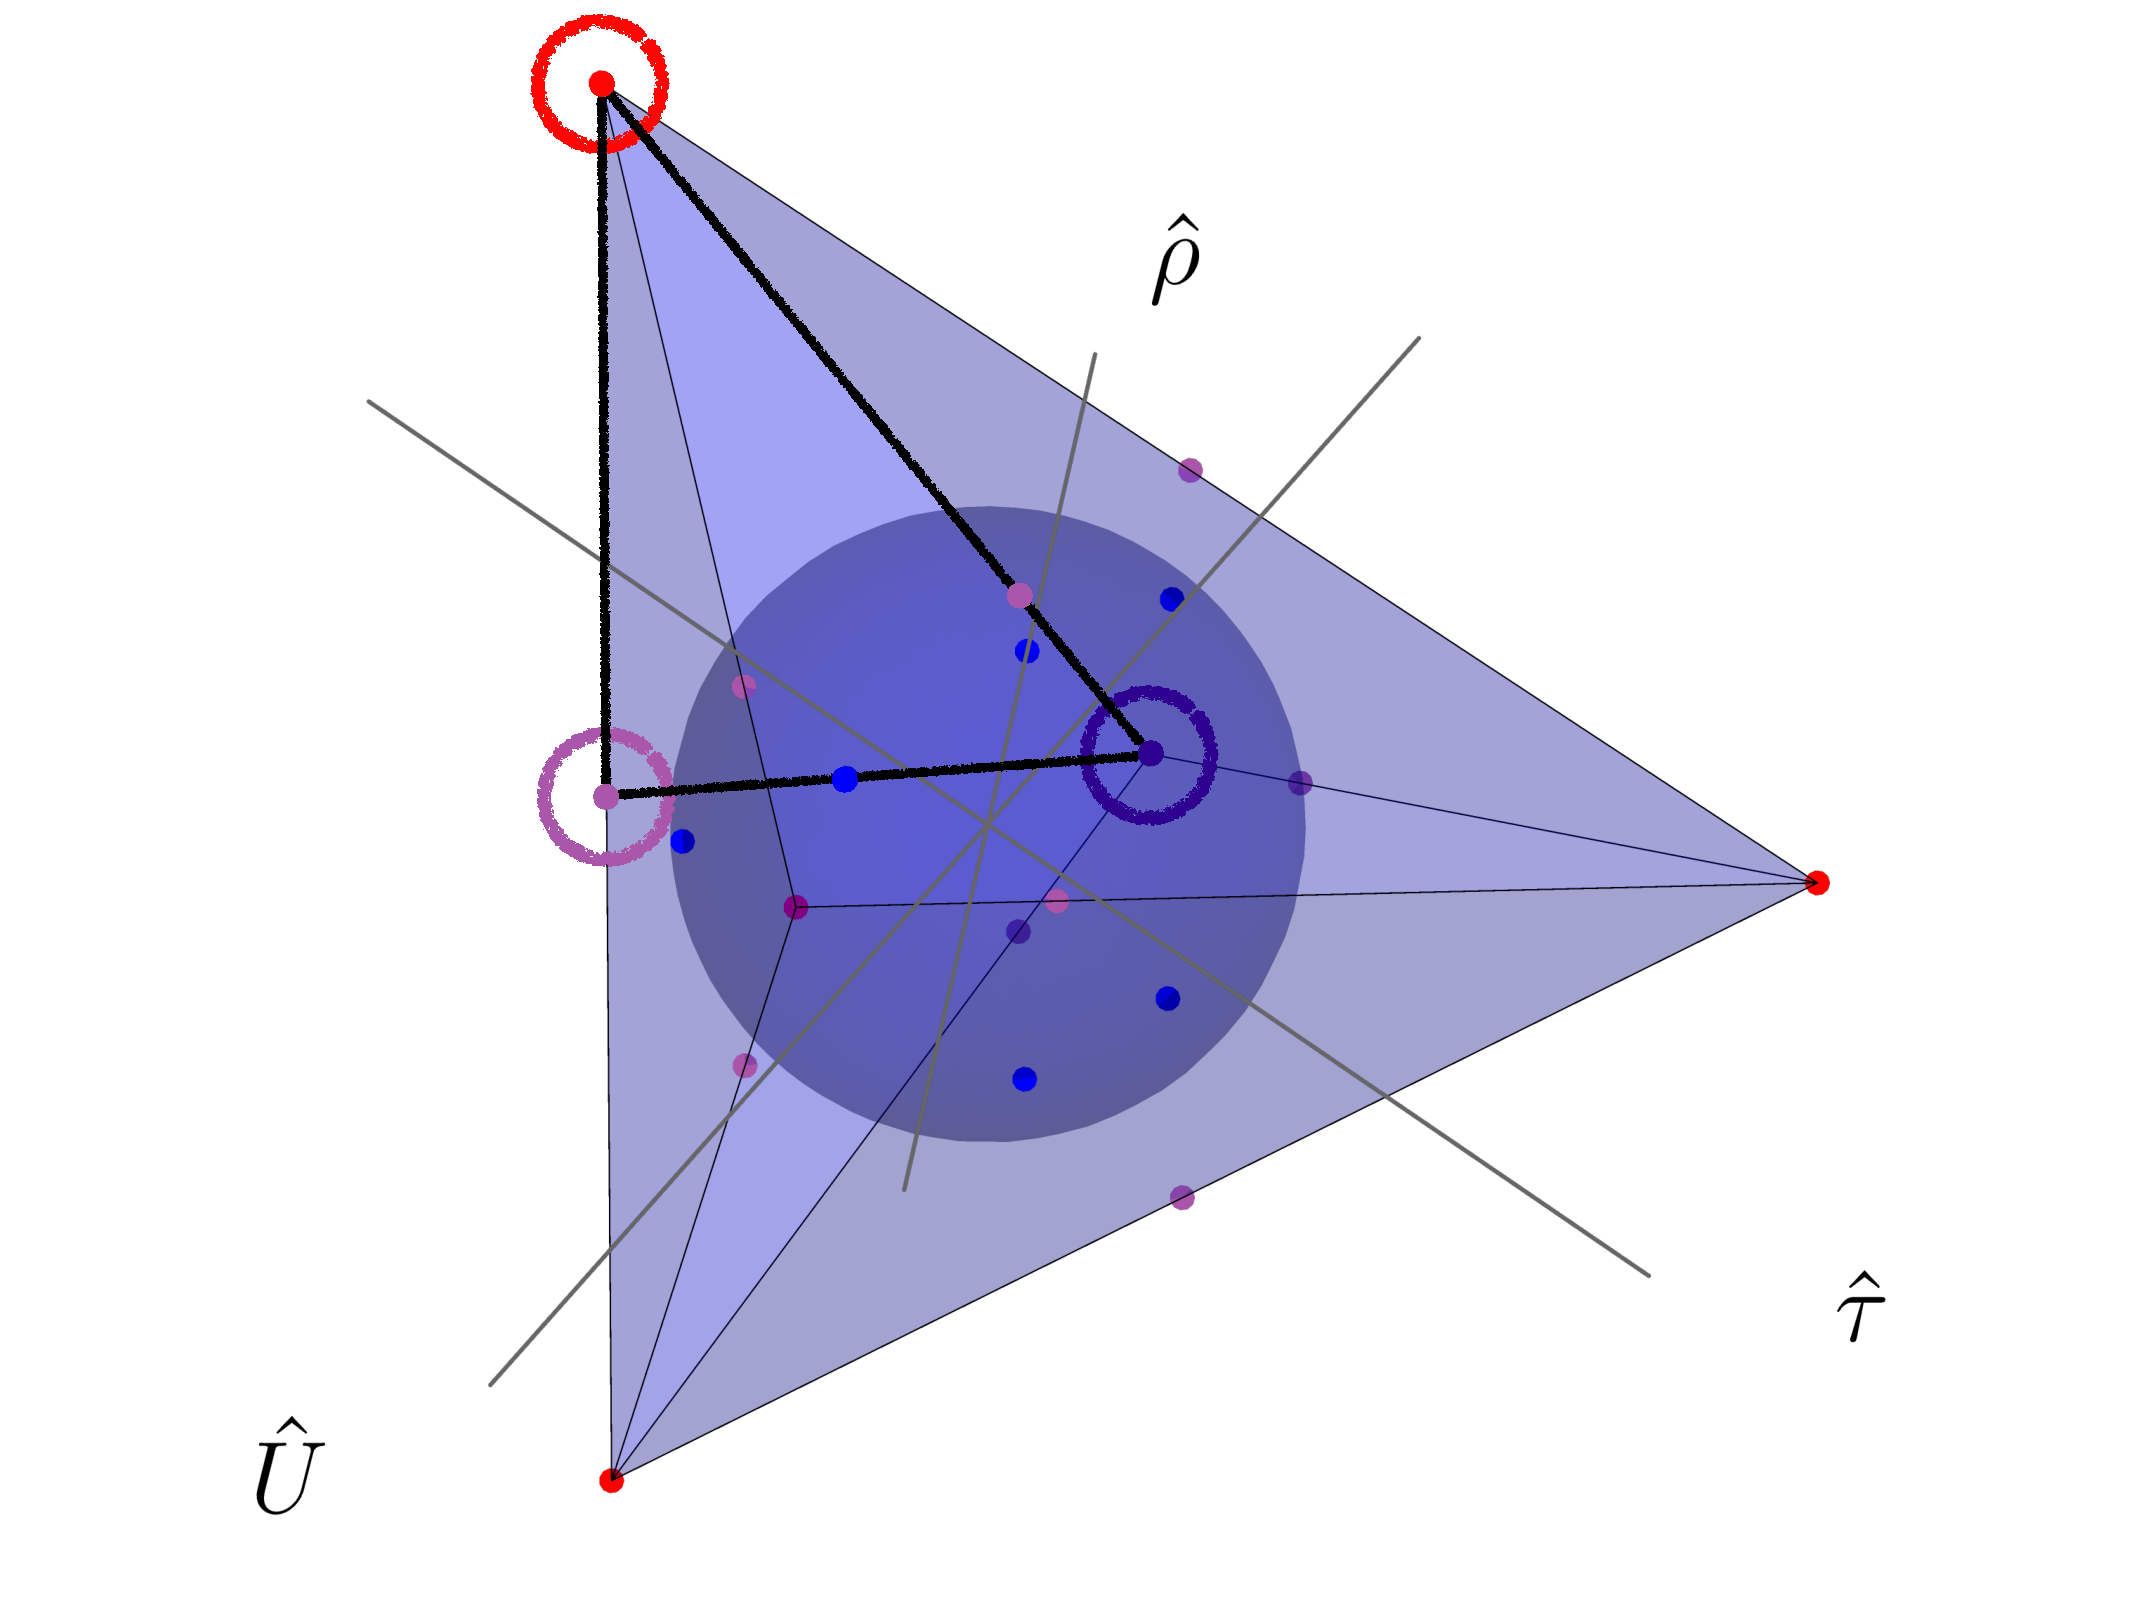
\includegraphics[width=0.45\textwidth]{CH-T3-1v2.pdf}
			}
			\subfigure{
				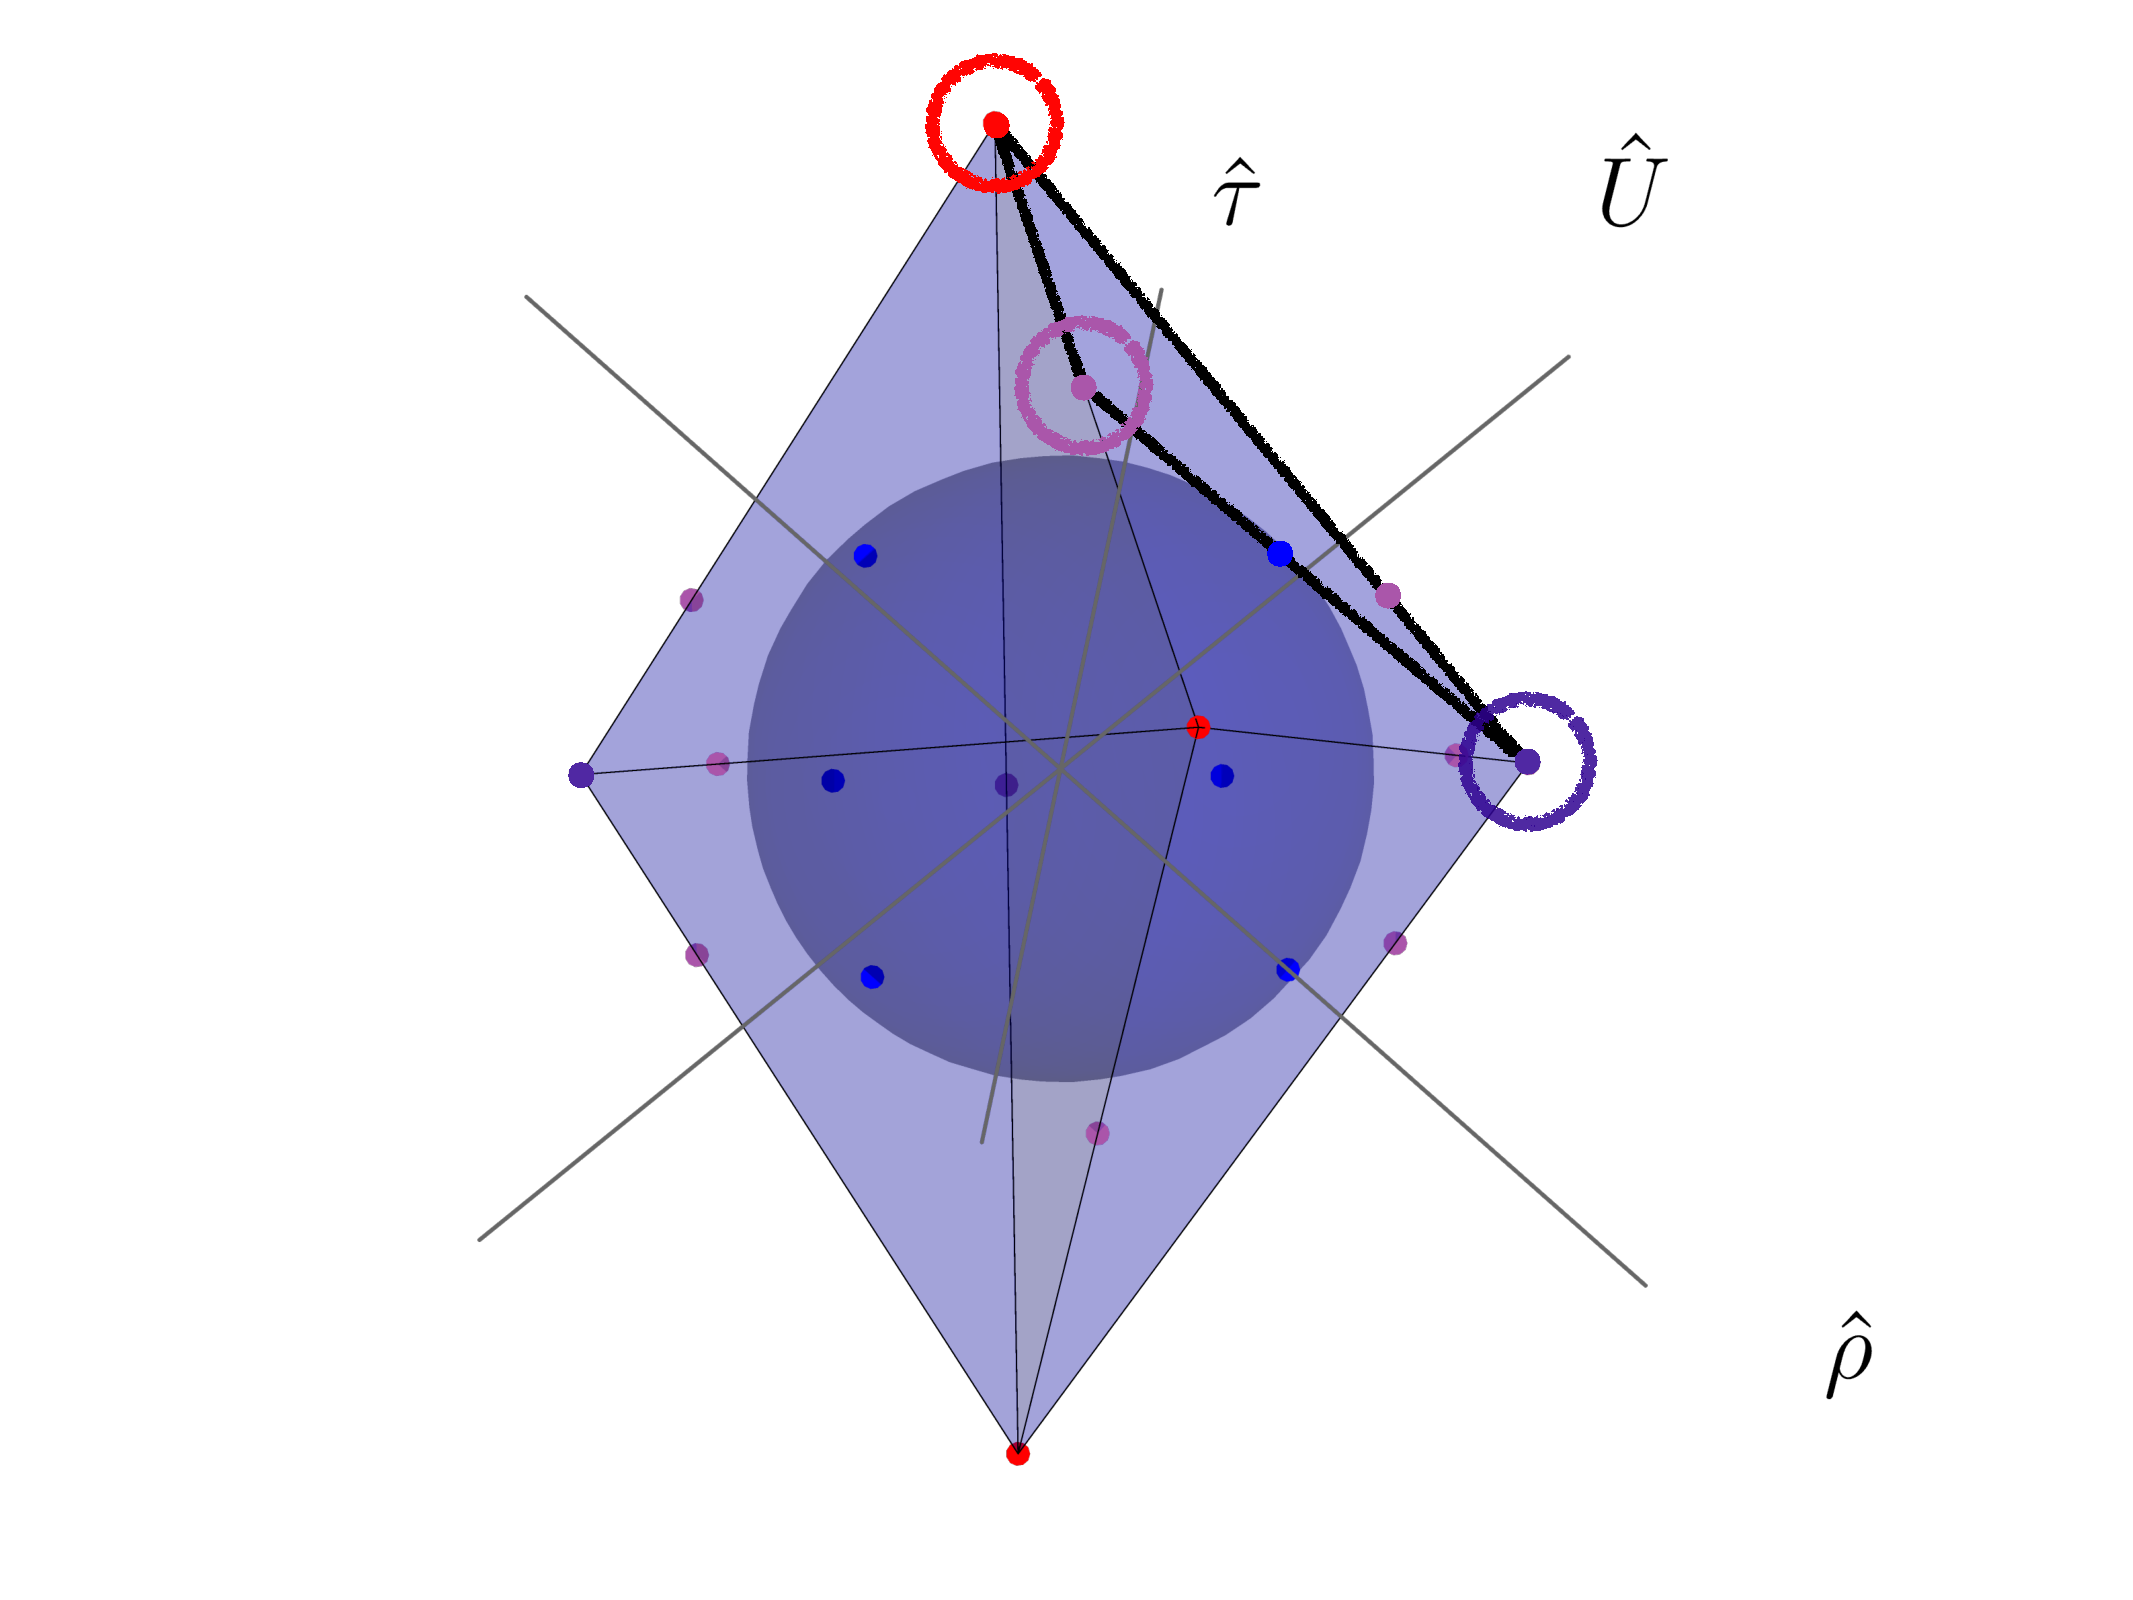
\includegraphics[width=0.45\textwidth]{CH-T3-2v2.pdf}
			}
			\caption{\small Phase diagram for the (asymptotic) species scale in M-theory on $\mathbf{T}^3$, as seen from two different angles. The axes correspond to the canonical variables $\lbrace \hat U = \frac{3}{\sqrt{14}} \log \mathcal{V}_2\, ,\, \hat \tau= \frac{1}{\sqrt{2}}\log \tau_2\, ,\, \hat \rho = \sqrt{\frac76} \log R_3\rbrace$. The blue dots are associated to circle decompactifications, the light purple ones signal some double decompactification to 10d, whilst the purple and red dots correspond to full decompactification to 11d and emergent Type II string limits, respectively. We have selected three particular directions which span a cone determining some fundamental domain $\mathscr{F}_8$.}
			\label{fig:MthyT3}
		\end{center}
\end{figure} 
%%%%%%%%%%%%%%%%%

Before proceeding any further, let us note that if instead of the $\lbrace \nu, \tau\rbrace$--\,parametrization one chooses the alternative $\lbrace \varphi_8, T\rbrace$ coordinates --- whose leading order action is shown in eq. \eqref{eq:8dIIB}, the $\mathsf{SL(3,\mathbb{Z})}$--\,series can be expanded as follows
%
\begin{align}\label{eq:Eisenstein3/2-2ap}
	\hat{E}_{3/2}^{sl_3} &= 2\zeta(3) e^{-2\varphi_8} + 2 \hat{E}_{1}^{sl_2} (T) + \frac{4 \pi}{3} \varphi_8 + \mathcal{O} \left( \exp(-e^{-\varphi_8})\right)\, ,
\end{align}
%
which of course agrees with \eqref{eq:instexpSL3ap}.

In order to connect with our discussion in the M-theory picture, we need to rewrite the previous $\mathcal{R}^4$ correction in terms of the variables adapted to the action \eqref{eq:8dalternativeactionII}. Hence, upon using the map between Type IIB and M-theory (c.f. Section \ref{s:dualities})
%
\begin{center}
\renewcommand{\arraystretch}{2.00}
\begin{tabular}{r c l}
M-theory on $\mathbf{T}^3$ & $\longleftrightarrow $ & Type IIB on $\mathbf{T}^2$\\ 
\hline
\hline  
$\mathcal{T}$ & $ \longleftrightarrow$ & $U$ \\
$\tau$ & $\longleftrightarrow $&  $T$\\
$\mathcal{V}_2^{9/7}\, R_3^{-2}$ & $\longleftrightarrow $ & $e^{-2\varphi_8}$
\end{tabular}\label{tab:8dMthy/IIB}
\end{center}  
%
as well as the expression for the $\mathbf{T}^3$ volume in terms of $\mathcal{V}_2$ and $R_3$ (see eq. \eqref{eq:T3volume}), one finds
%
\begin{equation} \label{eq:usefulmap}
      \mathcal{V}_2 = T_2^{\frac{2}{3}}\, e^{-\frac{2\varphi_8}{3}}\, , \qquad R_3 = T_2^{\frac{3}{7}}\, e^{\frac{4\varphi_8}{7}}\, .
\end{equation}
%
From these we can also deduce how the Type IIB coordinate $\nu$ relates to the M-theory variables, namely $\nu=\mathcal{V}_2^{-18/7}\, R_3^4\, \tau_2^{-3/2}$, thus allowing us to rewrite the first few terms in $\hat{E}_{3/2}^{sl_3}$ as
%
\begin{align}\label{eq:instexpSL3Mth1}
	\hat{E}_{3/2}^{sl_3} &= 2\zeta(3) \mathcal{V}_2^{9/7}\, R_3^{-2} + \frac{2\pi^2}{3} \tau_2 - 2\pi \text{log} (\tau_2) - \frac{2 \pi}{3} \log \left( \mathcal{V}_2^{9/7}\, R_3^{-2}\right) + \ldots\, ,
\end{align}
%
where the ellipsis indicates further non-perturbative contributions.


\subsubsection*{Asymptotic checks}

With this information, we are now ready to analyze whether the moduli-dependent Wilson coefficient associated to the  $t_8 t_8 \mathcal{R}^4$ operator in \eqref{eq:8dR^4IIB} exhibits the behaviour predicted by \eqref{eq:scalargravDlag}. To do so, we follow the same procedure as in the 9d example from Section \ref{ss:MthyT2}, therefore studying different representative infinite distance limits within $\mathcal{M}_{\rm 8d}$. Importantly, notice that by U-duality we can actually restrict ourselves to some fundamental domain $\mathscr{F}_8$ containing the minimal non-redundant information captured by the asymptotic phase diagram shown in Figure \ref{fig:MthyT3} above.\footnote{In Part \ref{part:pattern} of the thesis we will explain how to systematically construct such fundamental domains by looking precisely at the tangent bundle of the moduli space, see in particular the discussion in Section \ref{sss:sketch}.} For concreteness, we take a cone within $\mathcal{M}_{\rm 8d}$ spanned by geodesic directions associated to \emph{(i)} some emergent Type II string limit, \emph{(ii)} a pure decompactification to 10d (implementing M/F-theory duality) \emph{(iii)} as well as a third direction involving full decompactification to 11d M-theory. In particular, using an orthonormal frame adapted to the non-compact scalar fields appearing in \eqref{eq:8dalternativeactionII}, the aforementioned region corresponds to the cone generated by the following three directions in Figure \ref{fig:MthyT3}: one red dot at a vertex (emergent string limit), one purple dot at other vertex sharing a common edge with the former (decompactification to 11d), and finally one light purple dot (decompactification to 10d) belonging to the same facet as the other two and sharing an edge with the red dot but not with the purple one. Note that any such domain automatically includes additional asymptotic directions associated to yet another partial decompactification of two extra dimensions (light purple dot), and one partial decompactification of some $\mathbf{S}^1$ within the $\mathbf{T}^3$ (blue dot at the interior of the cone). A specific choice for $\mathscr{F}_8$ is shown in Figure \ref{fig:MthyT3}, which in 8d M-theory variables $\lbrace \tau_2, R_3, \mathcal{V}_2 \rbrace$ is defined by the following inequalities
%
\begin{equation}
    \label{eq:funddomainT3}
\mathcal{V}_2^{9/7} \, R_3^{-2}\,  \geq\, \tau_2\, \geq 1 \, ,  \qquad \mathcal{V}_2 \geq R_3^{-7/6} \, .
\end{equation}
%
Moreover, the three limiting directions spanning the cone \eqref{eq:funddomainT3} correspond to the following asymptotic species scales (in 8d Planck units) 
%
\begin{equation} \label{eq:QGcutoffs8d}
	\begin{split} 
		\frac{m_{\text{str}}}{M_{\rm Pl;\, 8}} &= \frac{(4\pi)^{1/3}}{\sqrt{2}} R_3^{1/3}\, \mathcal{V}_2^{-3/14} \, , \qquad \frac{M_{\rm Pl;\, 10}}{M_{\rm Pl;\, 8}} = (4\pi)^{1/24} R_3^{1/12}\, \mathcal{V}_2^{-3/56}\, \tau_2^{-1/8} \, ,\\
		\frac{M_{\rm Pl;\, 11}}{M_{\rm Pl;\, 8}} &= (4\pi)^{-1/18} R_3^{-1/6}\, \mathcal{V}_2^{-1/7} = (4\pi)^{-1/18} \mathcal{V}_3^{-1/6}\, ,
	\end{split}
\end{equation}
%
which eq. \eqref{eq:8dR^4IIB} should reproduce upon taking appropriate limits within $\mathscr{F}_8$. We study each of them in turn. %These correspond to the mass scale of a fundamental Type II string, as well as the 10d and 11d Planck masses of dual F-/M-theory descriptions.
\newline

\underline{\textit{The M-theory regime}}
\newline

Let us first consider the asymptotic regime of the selected fundamental domain where $M_{\rm Pl;\, 11}$ is the lightest of these three scales, and therefore fixes the species cut-off, i.e. $\LSP=M_{\rm Pl;\, 11}$. Geometrically, this corresponds to the $\mathbf{T}^3$ decompactification limit $\mathcal{V}_3 \to \infty$ with $\mathcal{V}_2 \leq R_3^7$, restricted to \eqref{eq:funddomainT3}. It is moreover associated to the $\mathsf{SL(2,\mathbb{Z})}$ sector of the theory, since the $\hat{E}_{1}^{sl_2}$ term within \eqref{eq:8dR^4IIB} clearly dominates. Hence, for all such limits we find (c.f. eq. \eqref{eq:asymptotic behavior})
%
\beq
2\hat{E}_{1}^{sl_2}(\mathcal{T}, \bar{\mathcal{T}}) = -2\pi\text{log} \left(\mathcal{T}_2\,|\eta(\mathcal{T})|^4\right)\, \sim\, \frac{\pi^2}{3} \mathcal{V}_3\, \propto\, \left(\frac{M_{\rm Pl;\, 11}}{M_{\rm Pl;\, 8}}\right)^{-6}\, ,
\eeq
%
where the asymptotic dependence should be understood when taking limit $\mathcal{T}_2\to \infty$. This matches exactly with eq. \eqref{eq:scalargravDlag}, thus recovering the expected suppression of the $\mathcal{R}^4$--\,term with $\LSP^6$.
\newline

\underline{\textit{The Type II regime}}
\newline
 
The asymptotic region in which the Type II fundamental string scale is the lightest within $\mathscr{F}_8$ is given by $\mathcal{V}_2 \geq R_3^7$, and hence corresponds to $\LSP=m_{\text{str}}$. In this regime, the leading contribution to \eqref{eq:8dR^4IIB} comes from the order--$\frac32$ $\mathsf{SL(3,\mathbb{Z})}$ Eisenstein series, such that all encompassing asymptotic boundaries are mapped to the limit $\nu \to \mathcal{V}_2^{-18/7}\, R_3^4\, \tau_2^{-3/2}\to 0$ in the Type IIB dual frame (see discussion around eq. \eqref{eq:usefulmap}). Thus, upon using the expansion \eqref{eq:instexpSL3Mth1}, one obtains the following leading order contribution to the $\mathcal{R}^4$--\,operator
%
\begin{align}
\label{eq:8dtotypeII}
	\hat{E}_{3/2}^{sl_3}\, \sim\, 2\zeta(3) \mathcal{V}_2^{9/7}\, R_3^{-2}\, \propto\, \left(\frac{m_{\text{str}}}{M_{\rm Pl;\, 8}}\right)^{-6}\, ,
\end{align}
%
which in turn reproduces the expected suppression with the species scale.
\newline

\underline{\textit{Decompactification to 10d}}
\newline

Note that the two regimes described so far already cover the entire asymptotic region associated to the fundamental domain defined in \eqref{eq:funddomainT3}. However, along certain directions, one may actually find additional partial decompactification limits, as we discuss in what follows. For instance, within the selected domain, the region where the 10d Planck mass sets the species cut-off corresponds to the boundary where it coincides with the string scale, namely $\tau_2=\, \mathcal{V}_2^{9/7}\, R_3^{-2}$ and $\mathcal{V}_2 \geq R_3^7$. In that case, the mass scale of the (double) KK tower represented by the light purple dot in Figure \ref{fig:MthyT3} is actually lighter than the string scale. Thus, what we end up seeing is actually a decompactification to ten dimensions, with the 10d Planck mass being parametrically of the same order as the string scale, i.e. $\LSP=M_{\rm Pl;\, 10}\sim m_{\text{str}}$. The dominant contribution to the $\mathcal{R}^4$ term thus takes the same form as in eq. \eqref{eq:8dtotypeII}, which can be equivalently expressed as
%
\beq
\hat{E}_{3/2}^{sl_3}\, \sim\, \left(\frac{M_{\rm Pl;\, 10}}{M_{\rm Pl;\, 8}}\right)^{-6} \, ,
\eeq
%
in agreement with \eqref{eq:scalargravDlag}.
\newline

\underline{\textit{Decompactification to 9d}}
\newline

Finally, we study the special direction corresponding to the center of the facet within $\mathscr{F}_8$, to which we can associate a single KK tower signalling decompactification from 8d to 9d as shown in Figure \ref{fig:MthyT3}. Furthermore, this asymptotic geodesic, which is parametrized by $\tau_2=\mathcal{V}_2=R_3^7 \to \infty$, is such that all potential candidates for the species cut-off in eq. \eqref{eq:QGcutoffs8d} scale in the same way. Hence, along this limit, we have 
%
\begin{equation}
   \hat{E}_{3/2}^{sl_3}\, \sim\, \hat{E}_{1}^{sl_2}\, \sim\,  \left(\frac{M_{\rm Pl;\, 9}}{M_{\rm Pl;\, 8}}\right)^{-6} \, ,
\end{equation}
%
yielding once again the correct dependence with the number of species for the $\mathcal{R}^4$--\,term.

All in all, we conclude that the function 
%
\beq
\LSP = \left( \hat{E}_{3/2}^{sl_3} +2\hat{E}_{1}^{sl_2}\right)^{-1/6}\, ,
\label{eq:8dfullspeciesfn}
\eeq
%
captures every single relevant asymptotic behaviour of the species scale in 8d maximal supergravity, as arising from e.g., M-theory compactified on $\mathbf{T}^3$. It is moreover invariant under the $\mathsf{SL(2,\mathbb{Z})}\times \mathsf{SL(3,\mathbb{Z})}$ duality group and thus reproduces precisely the phase diagram depicted in Figure \ref{fig:MthyT3}.

Before closing this section, let us remark that one can also consider higher order curvature corrections to the 8d effective action and perform a similar analysis, since some of these terms have been already computed in the literature (see e.g., \cite{Green:2010wi}). Upon doing so, one finds, similarly to the previous examples in ten and nine dimensions, that they are not in general suppressed by the appropriate power of the species scale, at least for certain type of limits (i.e. decompactification limits), but rather by the scale associated to the lightest tower. A potential physical explanation for this discrepancy will be explained later on in Section \ref{ss:gravEFTexpansion}. %, but for the moment let us stress one more time that we believe the $\mathcal{R}^4$--\,correction to be the one capturing the UV divergence of the eight-dimensional EFT related to the species scale.


\section{String theory examples in lower dimensions}
\label{s:4dN=2}

In this section we will focus on 4d $\mathcal{N}=2$ settings arising from Type IIA string theory compactified on a Calabi--Yau three-fold $X_3$. Such theories are known to present, beyond the two-derivative lagrangian discussed in Section \ref{sss:4dN=2basics}, interesting higher-dimensional and higher-curvature corrections. In particular, there is an infinite number of F-terms, which are $\frac{1}{2}$-BPS and thus protected by supersymmetry, ensuring that their dependence with respect to the vector multiplet moduli can be computed in an exact manner. They read as follows \cite{Bershadsky:1993ta, Bershadsky:1993cx,Antoniadis:1993ze,Antoniadis:1995zn}:
%
\beq
\label{eq:lagrangian}
	S_{\text{IIA}}^{\text{4d}} \supset \int \dd^4x\, \sqrt{-g}\, \int \dd^4\theta\, \sum_{g\geq 1} \mathcal{F}_g (\mathcal{X}^A)\, \mathcal{W}^{2g}\ +\ \text{h.c.}\, ,
\eeq
%
where $\mathcal{F}_g (\mathcal{X}^A)$ is a chiral superfield that is related to the $g$-loop topological free energy of the supersymmetric closed string, $\theta^{\alpha}$ denote the fermionic $\mathcal{N}=2$ superspace coordinates and $\mathcal{W}_{\mu \nu} = F^+_{\mu \nu} - \mathcal{R}^+_{\mu \nu \rho \sigma} \theta \sigma^{\rho \sigma} \theta + \ldots\,$, is the Weyl superfield, which in Euclidean signature depends on the self-dual components of the graviphoton field strength and the Riemann tensor \cite{Antoniadis:1995zn}. Thus, upon performing the integration over the fermionic variables, one finds terms within \eqref{eq:lagrangian} of the form
%
\beq
\label{eq:GVterms}
	S_{\text{IIA}}^{\text{4d}} \supset \int \dd^4x\, \sqrt{-g}\, \left( \sum_{g\geq 1} \mathcal{F}_g(X^A)\, \mathcal{R}_+^2\, F_+^{2g-2} \right)\ +\ \text{h.c.}\, ,
\eeq
%
where $X^A$, $A=0,\ldots, h^{1,1}$, denote the bottom (i.e. scalar) components of the chiral superfields $\mathcal{X}^A$, c.f. eq. \eqref{eq:projcoords}.

As originally proposed in \cite{Gopakumar:1998ii,Gopakumar:1998jq}, one can alternatively compute the quantities $\mathcal{F}_g$ for $g\geq 0$ using the duality between Type IIA string theory on $X_3$ and M-theory on $X_3 \times \mathbf{S^1}$. For a single BPS particle of mass $m=|Z|$ --- where $Z$ denotes its central charge, one indeed obtains a generating function via a Schwinger-type one-loop computation in the presence of a constant self-dual graviphoton background, as follows
%
\begin{align}
\label{eq:generatingseries}
	\notag \sum_{g\geq 0}\mathcal{F}_g\, F_+^{2g-2} &= -\frac{1}{4} \int_{0^+}^{i \infty}\frac{\dd\tau}{\tau} \frac{1}{\sin^2{\frac{\tau F_+ \bar Z}{2}}} e^{-\tau m^2}\\
    &= \frac{1}{4} \int_{0^+}^{\infty}\frac{\dd\tau}{\tau} \sum_{g\geq0} \frac{2^{2g} (2g-1)}{(2g)!} (-1)^{g} B_{2g} \left( \frac{\tau F_+}{2}\right)^{2g-2} e^{-\tau Z}\, +\, \mathcal{O}\left(e^{-\frac{Z}{F_+}}\right)\, ,
\end{align}
%
where in the second step we rotated the integration contour %have changed the integration variable $\tau \to \tau /\bar Z$
and we have performed a perturbative expansion using the Laurent series for $\csc^2(x)$ around zero, namely
%
\begin{align}
	\frac{1}{\sin^{2}(x)} = \sum_{n=0}^{\infty} \frac{2^{2n}(2n-1)}{(2n)!} (-1)^{n-1} B_{2n} x^{2n-2}\, ,
\end{align}
%
which is valid for $0<|x|<\pi$. Notice that the coupling of the BPS particle to the background field crucially involves the anti-holomorphic piece of the mass \cite{Dedushenko:2014nya}. The $B_{2g}$ are referred to as Bernouilli numbers, which are given by
%
\begin{align}\label{eq:bernouilli}
	B_{2g}= \frac{(-1)^{g+1} 2 (2g)!}{(2\pi)^{2g}} \zeta(2g)\, .
\end{align}
%
From eq. \eqref{eq:generatingseries} one may already get a feeling of which $\mathcal{F}_g$ are UV sensitive/divergent versus those which actually provide for a convergent contribution. The claim would be that for $g\geq2$, the above integral converges in the UV, whilst for $g=0,1,$ one needs to adopt some regularization scheme. Indeed, one finds
%
\begin{align}
\label{eq:divergence}
	\mathcal{F}_g \propto \int_{\varepsilon}^{\infty} \dd\tau\, \tau^{2g-3}e^{-\tau Z} = Z^{2-2g} \Gamma(2g-2, \varepsilon Z)\, ,
\end{align}
%
where $\varepsilon=\Lambda_{\rm UV}^{-2}$ is nothing but the Schwinger implementation of the UV cut-off. Therefore, for $g > 1$, the incomplete gamma function converges to $\Gamma(2g-2) = (2g-3)!\,$, whilst for the remaining cases one finds a UV divergence that needs to be carefully dealt with.

In what follows, we will study the moduli dependence of the coefficients $\mathcal{F}_g(X^A)$ when probing certain representative infinite distance limits within the vector multiplet moduli space \cite{Lee:2019wij}.\footnote{The quantities $\mathcal{F}_g$, as computed by the topological string theory, are holomorphic in the chiral coordinates $\mathcal{X}^A$. There exists, however, a holomorphic anomaly in the quantum effective action associated to the contribution of the massless fields \cite{Bershadsky:1993cx}. For our purposes here, it will be enough to focus just on the holomorphic piece.} We will distinguish between operators that are relevant/marginal (in the Wilsonian sense), from those which are irrelevant (and thus UV convergent). The focus will be placed on understanding whether the general EFT expansion proposed in \eqref{eq:scalargravDlag} is fulfilled or not in the present 4d set-up.

\subsection{The $\mathcal{R}^2$--\,operator}
\label{ss:threshold4d}

Let us start with the only relevant/marginal BPS operator within the 4d lagrangian \eqref{eq:GVterms}, i.e. the one associated to $g=1$. It is proportional (in Euclidean signature) to the self-dual part of the curvature tensor squared, and its Wilson coefficient can be identified with the A-model topological free energy at genus one. In what follows, we review the mathematical definition and basic properties of $\mathcal{F}_1$, as computed from the topological string side.

This quantity can be defined as a supersymmetric index in the $\mathcal{N}=(2,2)$ superconformal field theory (SCFT) living on the worldsheet \cite{Cecotti:1992vy,Cecotti:1993stu}
%
\begin{align}
\label{eq:defF_1}
	\mathcal{F}_1 = \frac12 \int_{\mathscr{F}} \frac{\dd^2\tau}{\tau_2}\, \text{tr} \left( (-1)^F\, F_L\, F_R\, e^{2\pi \i H_0}\, e^{-2\pi \i \bar{H}_0}\right)\, ,
\end{align}
%
where $F_{L(R)}$ corresponds to the left-(right-)moving fermion number in the 2d theory, $F= F_L+F_R$ and $H_0$ denotes the associated Hamiltonian. Actually, the above index turns out to be IR divergent due to the contribution of the string massless states, and thus it should be properly regularized. This prescription only determines $\mathcal{F}_1$ up to an overall additive constant. Moreover, despite the apparent holomorphicity on the background flat coordinates $\{t^i\}$ --- i.e. the vector multiplet moduli, there is in fact some holomorphic anomaly which is captured by the following differential equation 
%
\begin{align}
\label{eq:holoanomalyF1}
	\frac{\partial^2\mathcal{F}_1}{\partial t^i \partial \bar{t}^j} = \text{tr}\, (-1)^F C_i \bar{C}_{\bar{j}} - \frac{1}{12} G_{i \bar{j}}\, \text{tr}\, (-1)^F\, ,
\end{align}
%
with $C_i (\bar{C}_{\bar{j}})$ being the structure constants of the (anti-)chiral ring of supersymmetric ground states and $G_{i \bar{j}}$ denotes the moduli space metric (see \cite{Bershadsky:1993ta} for details). Importantly, the above equation can be integrated exactly, thus fixing the moduli dependence of $\mathcal{F}_1$ up to some holomorphic function $f(t^i)$ that can be determined by confronting the solution to \eqref{eq:holoanomalyF1} with its expected boundary behaviour \cite{Bershadsky:1993ta,Bershadsky:1993cx}. The resulting expression would read as
%
\beq\label{eq:F1IIA}
	\mathcal{F}_1 =   \frac {1}{2}\left( 3+h^{1,1}-\frac {\chi_{E} (X_3)}{12}\right)K_{\text{ks}} + \frac {1}{2}\log \det G_{i \bar j} + \log|f|^2\, ,
\eeq
%  
where $\chi_E(X_3)$ is the Euler characteristic of the three-fold $X_3$, whilst $K_{\text{ks}}$ denotes the K\"ahler potential for the moduli fields. Crucially, it turns out that the asymptotic properties exhibited by $\mathcal{F}_1$ indeed match the behaviour predicted by \eqref{eq:scalargravDlag}, where one should take into account that the corresponding $\mathcal{R}^2$--operator has mass dimension $n=4$, such that we expect the above quantity to behave like 
%
\beq\label{eq:F1QGcutoff}
	\mathcal{F}_1\, \sim\, \left(\frac{\Mpf}{\LSP}\right)^2\, .
\eeq
%
For illustrative purposes, let us briefly consider Type IIA string theory compactified on the Enriques Calabi--Yau $\left(K3 \times \mathbf{T}^2\right)/\mathbb{Z}_2$ \cite{Klemm:2005pd}, which is known to be dual to a Heterotic compactification on $K3 \times \mathbf{T}^2$. In this case, one finds that the moduli space metric behaves as $G_{T \bar{T}}=\frac{1}{4 T_2^2}\, $ (at large volume), whereas the genus-one topological free energy takes the following simple form \cite{vandeHeisteeg:2023ubh,Grimm:2007tm}
%
\beq \label{4dtopologicalfreeenergy}
\mathcal{F}_1 =-6 \log \left( T_2 |\eta(T)|^4\right) + \text{const.}\, , 
\eeq
%
where $T$ denotes the complexified K\"ahler modulus of the internal torus. In the original Type IIA frame, an emergent string limit arises when taking $T_2 \to \infty$ --- corresponding to a large volume limit for the internal $\mathbf{T}^2$, where the critical string is featured by a NS5-brane wrapping the $K3$-fibre, with tension
%
\beq
	T_{\rm NS5,\, str} = \frac{\Mpf^2}{2T_2}\, .
\label{eq:hettensionEnriques}
\eeq
%
In the dual Heterotic frame, such infinite distance degeneration is mapped to a perturbative weak coupling point for the fundamental string. Therefore, upon using eq. \eqref{eq:asymptotic behavior} we find
%
\beq
\mathcal{F}_1 =2\pi T_2 + \mathcal{O}\left( \log T_2\right)\, , 
\eeq
%
which is in perfect agreement with \eqref{eq:F1QGcutoff} above.

Let us remark here that an analysis along these lines can be analogously performed when probing other kind of infinite distance limits within the vector multiplet sector of 4d $\mathcal{N}=2$ theories, including partial decompactifications to M-/F-theory, see below. This was done in detail in refs. \cite{vandeHeisteeg:2022btw,vandeHeisteeg:2023ubh}, so we refrain from repeating it here and refer the interested reader to the original works.

\subsection{The irrelevant operators}
\label{ss:UVconvergent}

We turn now to the BPS operators in eq. \eqref{eq:GVterms} with $g>1$. Using eq. \eqref{eq:generatingseries}, we find that the contribution to $\mathcal{F}_{g>1}$ due to a particle of mass $m= |Z|$ is
%
\begin{equation}
\label{eq:Fg>1}
	\mathcal{F}_{g>1}= \frac{(2g-1)}{(2g)!} (-1)^g B_{2g} \int_0^{\infty} \dd\tau\, \tau^{2g-3}e^{-\tau Z}\, ,
\end{equation}
%
where one should substitute the appropriate Bernouilli numbers from \eqref{eq:bernouilli}. In the following, we will extract the relevant asymptotic behaviour of these higher-dimensional operators depending on the infinite distance limit that we approach. Later on, in Section \ref{ss:gravEFTexpansion} we comment on how these examples fit within the general framework discussed in Chapter \ref{ch:SpeciesIntro}.

\subsubsection*{M-theory limit}

The large volume point (with 4d dilaton fixed and finite) corresponds to a decompactification limit to 5d M-theory, where the M-theory circle grows large. This can be easily understood by looking at the light spectrum of the theory along the aforementioned limit, where it is precisely the tower of D0-branes which become light the fastest (see e.g., \cite{Font:2019cxq}). These states are $\frac12$-BPS, with a mass given by
%
\begin{equation}
\label{eq:D0mass}
	m_n = 2\pi |n|\, \frac{m_s}{g_s} = |n|\, m_{\rm D0}\, ,
\end{equation}
%
where $m_s$ is the fundamental Type IIA string scale and $n\in \mathbb{Z} \setminus \{ 0\}$ denotes the D0-brane charge. Notice that we are excluding the contribution of the massless (i.e. $n=0$) fields here, which would be actually part to the 4d EFT. After substituting in \eqref{eq:Fg>1}, one finds
%
\begin{align}
\label{eq:Fg>1D0}
	\mathcal{F}^{\rm D0}_{g>1}&= \chi_E(X_3) \frac{(2g-1) \zeta(2g)}{(2\pi)^{2g}} \sideset{}{'}\sum_{n \in \mathbb{Z}}\int_0^{\infty}d\tau\, \tau^{2g-3}e^{-\tau\, n\,  m_{\rm D0}} \notag\\
    &=\chi_E(X_3) \frac{(2g-1) \zeta(2g)}{(2\pi)^{2g}} \Gamma(2g-2)  m_{\rm D0}^{2-2g} \sideset{}{'}\sum_{n \in \mathbb{Z}} \frac{1}{n^{2g-2}} \notag\\
    &= \chi_E(X_3)\frac{2(2g-1) \zeta(2g) \Gamma(2g-2)}{(2\pi)^{2g}} \frac{\zeta(2g-2)}{m_{\rm D0}^{2g-2}}\, ,
\end{align}
%
which is of course convergent and moreover depends solely on the mass scale of the infinite tower of states, namely $m_{\rm D0}$, instead of the UV cut-off given by the species scale.

\subsubsection*{Partial decompactification limits}

Let us next consider the possibility that our Calabi--Yau three-fold presents some elliptic fibration $\pi: X_3 \to B_2$ (for simplicity we assume it to be non-singular). This means, in particular, that there exists an infinite distance limit at large volume within the vector multiplet moduli space where the base of the fibration blows up, whilst the volume of the elliptic fibre remains constant. Such limit corresponds to a partial decompactification limit to 6d F-theory \cite{Lee:2019wij}, where a tower of bound states with arbitrary D2 and D0-brane quantum numbers become asymptotically light (in 4d Planck units). The mass spectrum for such tower reads
%
\begin{equation}
\label{eq:ellipticmass}
	m_{n,\omega} = \frac{2\pi m_s}{g_s} \left| \omega z+n\right|\, ,
\end{equation}
%
where $z$ is the K\"ahler modulus associated to the elliptic fibre and $(n,\omega) \in \mathbb{Z}^2$ correspond to D0 and D2-brane charge, respectively. To properly account for the effect of such a tower one needs to sum over the integer set $(\omega, n)$, yielding
%
\begin{align}
\label{eq:Fg>1elliptic}
	\mathcal{F}^{\rm ell}_{g>1} (z)&= \chi_E(X_3)(-1)^{g-1} \frac{(2g-1)B_{2g} \Gamma(2g-2)}{2(2g)!} m_{\rm D0}^{2-2g} \sideset{}{'}\sum_{(\omega,n) \in \mathbb{Z}^2} \left(\omega z+n \right)^{2-2g}\notag\\
    &=\chi_E(X_3)(-1)^{g-1} \frac{(2g-1)B_{2g} \Gamma(2g-2)}{2(2g)!} \frac{G_{2g-2}(z)}{m_{\rm D0}^{2g-2}}\, ,
\end{align}
%
where in the last equality we have introduced the holomorphic Eisenstein series 
%
\begin{align}
\label{eq:holoEisenstein}
	G_{2k}(z) = \sideset{}{'}\sum_{(\omega, n) \in \mathbb{Z}^2} \frac{1}{\left(\omega z +n \right)^{2k}}\, .
\end{align}
%
Notice that the resulting operator is modular invariant,\footnote{The particular case of $g=2$ is a bit subtle, since it appears to be proportional to $G_2(z)$ which by itself is not a modular form. However, the holomorphic anomaly \cite{Bershadsky:1993cx} crucially solves this problem by promoting $G_2(z)$ in eq. \eqref{eq:Fg>1elliptic} to its non-holomorphic cousin, namely $\tilde{G}_2 (z, \bar z)= G_2(z)- \frac{\pi}{\text{Im}\, z}$, which now has definite modular weight.} as one can see from the fact that the terms in the lagrangian \eqref{eq:GVterms} are homogeneous in the fields $X^A$ of degree $2-2g$, whose K\"ahler transformation is exactly compensated by that of the graviphoton background field strength $F^+_{\mu \nu}$. Indeed, the relevant $\mathsf{SL(2,\mathbb{Z})}$ transformation corresponds to some generalized (double) T-duality which acts on the K\"ahler modulus as follows
%
\begin{align}\label{eq:Tdualitytrans}
	&z \rightarrow \frac{a\, z + b}{c\, z+d}\,,\qquad \text{with}\ \ \mathcal{A}= \begin{pmatrix}
		a \quad  b\\c \quad  d
	\end{pmatrix} \in \mathsf{SL(2,\mathbb{Z})}\, ,
\end{align}
%
whilst the vectors get transformed linearly through the matrix $\mathcal{A}$, which is moreover embedded into the symplectic K\"ahler group $\mathsf{Sp(2h^{1,1}+2, \mathbb{Z})}$, thus leaving all the F-terms in \eqref{eq:GVterms} invariant.\footnote{In general, these transformations are more complicated and also take into account the non-trivial fibration structure of the three-fold. This involves promoting the (double) T-duality in \eqref{eq:Tdualitytrans} to a Fourier-Mukai transform \cite{Andreas:2004uf, Cota:2019cjx}.} Note that the scale suppressing the tower of BPS operators becomes again that of the D2-particles (equivalently D0-branes, since both have asymptotically the same mass), and not the quantum gravity cut-off.

\subsubsection*{Emergent string limits}

Finally, we come to analyze infinite distance points in the vector multiplet moduli space corresponding to emergent string limits. These arise when the Calabi--Yau three-fold exhibits some $K3/\mathbf{T}^4$-fibration \cite{Lee:2019wij}, with the leading tower of asymptotically light states being the excitation modes of a dual critical string obtained by wrapping a NS5-brane on the generic fibre. As a concrete example, we consider here Type IIA compactified on $\mathbb{P}^{1,1,2,8,12}[24]$, which has $h^{1,1}=3$, $h^{2,1}=243$ and moreover exhibits a $K3$-fibration over a $\mathbb{P}^1$-base. The triple intersection numbers are \cite{Hosono:1994ax}
%
\beq
	\mathcal{K}_{111}=8\, , \quad \mathcal{K}_{112}=2\, , \quad \mathcal{K}_{113}=4\, , \quad \mathcal{K}_{133}=2,\, \quad \mathcal{K}_{123}=1\, .
\label{eq:triplenumbers}
\eeq
%
Upon probing the limit $t_b \to \infty$, where we denote by $t_b:= t^2$ the K\"ahler modulus associated to the $\mathbb{P}^1$-base, one encounters an infinite distance boundary of the emergent string kind, as discussed before. The corresponding tension of the wrapped NS5-brane reads
%
\beq
	T_{\rm NS5,\, str} = \Mpf^2 \frac{\mathcal{V}_{K3}}{2\mathcal{V}}\, ,
\label{eq:hettension}
\eeq
%
where $\mathcal{V}_{K3} = \frac{1}{2} \mathcal{K}_{2ij} t^i t^j = (t^1)^2 + t^1 t^3$ denotes the (classical) volume of the generic fibre and $\mathcal{V}$ that of the three-fold. Along the aforementioned limit, the 4d theory admits a dual interpertation in terms of a perturbative (i.e. weak coupling) limit for an $\mathsf{E_8} \times \mathsf{E_8}$ Heterotic compactification on $K3 \times \mathbf{T}^2$, with some $\mathsf{SU(2)}$ bundle (of instanton number 12) embedded in each of the $\mathsf{E_8}$ factors and such that all non-abelian symmetries are higgsed. The remaining $\mathsf{U(1)}$ factors come from the 3 vector multiplets associated to the geometric $\{T,U\}$ moduli of the internal torus and the complex dilaton $S= \frac{1}{2}\left(\varrho + \i e^{-2\varphi_4}\right)$, with $\varrho$ being a compact scalar dual to the Neveu-Schwarz 2-form $B_2$; as well as the graviphoton. Moreover, in the dual frame, the quantities $\mathcal{F}_{g>1}$ arise at one-loop order in string perturbation theory \cite{Antoniadis:1993ze,Antoniadis:1995zn}.

Incidentally, the moduli dependence of all the relevant higher-derivative couplings can be encapsulated at once upon defining the generating function 
%
 \beq
    F(\lambda, T, U)= \sum_{g=1}^{\infty} \lambda^{2g} \mathcal{F}^{\rm het}_g(T,U)\, ,
 \eeq
%
for which a formal exact expression is available in the case of interest \cite{Marino:1998pg}
%
\beq
	F(\lambda, T, U) = \frac{1}{2\pi^2} \int_{\mathscr{F}} \frac{\dd^2\tau}{\tau_2} \left( \frac{G_4 G_6}{\eta^{24}} \sum_{\Gamma^{2,2}} q^{\frac12 |p_L|^2} \bar{q}^{\frac12 |p_R|^2}\right) \left[ \left( \frac{2\pi \i \lambda \eta^3}{\theta_1(\tilde \lambda| \tau)}\right)^2 e^{-\frac{\pi \tilde \lambda^2}{\tau_2}}\right]\, .
\label{eq:Fheteroticoneloop}
\eeq
%
Here $\mathscr{F}$ denotes the $\mathsf{SL(2,\mathbb{Z})}$ fundamental domain, $G_4(\tau)$ and $G_6(\tau)$ are holomorphic Eisenstein series (c.f. eq. \eqref{eq:holoEisenstein}), $\theta_1$ is the Jacobi theta function with characteristics $(1/2,1/2)$, and we have defined the quantities
%
\beq
	\tilde \lambda = \frac{p_R \tau_2 \lambda}{\sqrt{2T_2 U_2}}\, , \qquad q=e^{2\pi \i \tau}\, ,
\eeq
%
where $p_{L,R}$ are the right-/left-moving momenta along the torus: 
%
\begin{align}
   p_L&= \frac{1}{\sqrt{2T_2U_2}} \left( n_1 +n_2 \bar{T} + m_2 U +m_1 \bar{T}U\right)\, ,\notag \\
   p_R&= \frac{1}{\sqrt{2T_2U_2}} \left( n_1 +n_2 T + m_2 U +m_1 T U\right)\, .
\end{align}
%
The important point for us is that all Wilsonian couplings captured by $F(\lambda, T, U)$ arise at one-loop and are thus proportional to $(S-\bar S)^0$ when written in the string frame. Therefore, upon switching to the 4d Einstein frame and taking the perturbative string limit, namely when $S \to \i \infty$ --- for generic values of the moduli $\{ T,U\}$, the functions $\mathcal{F}_{g>1}$ behave as follows
%
\beq
	\mathcal{F}^{\rm het}_{g>1} \sim \Mpf^{2-2g}(\text{Im}\, S)^{g-1} \sim \left(m_{\text{str, het}}\right)^{2-2g}\, ,
\eeq
%
where $m_{\text{str, het}}$ denotes the fundamental Heterotic string scale. In the original Type IIA description, this means that upon probing the limit $t_b \to \infty$, one finds
%
\beq \label{eq:F_g>1emergentstring}
	\mathcal{F}^{\rm IIA}_{g>1} \sim \Mpf^{2-2g} t_b^{g-1} \sim (T_{\rm NS5, \, str})^{1-g}\, ,
\eeq
%
with $T_{\rm NS5,\, str}$ given in eq. \eqref{eq:hettension} above. In this case, the scale suppressing the F-terms \eqref{eq:GVterms} does coincide with the species scale along the limit $t_b \to \infty$, since the latter is given by the (emergent) Heterotic string scale. Still, the particular power exhibited by \eqref{eq:F_g>1emergentstring} does not seem to agree with the expectations coming from eq. \eqref{eq:scalargravDlag}.

\subsection{General lessons}
\label{ss:gravEFTexpansion}

After the previous general considerations, we are now in good position to discuss the asymptotic mass dependence of the irrelevant F-terms appearing in generic 4d $\mathcal{N}=2$ theories arising from quantum gravity. We argue in the following that the relevant UV scale suppressing these terms in the EFT is the characteristic mass of the tower, such that the series expansion reads
%
\beq
\mathcal{L}_{\mathrm{IIA}}^{\text{4d}} \supset \sqrt{-g} \left(\sum_{n > 4} \frac{\mathsf{O}_n (\mathcal{R})}{m_{\rm tow}^{n-4}} \right) \, ,
\label{eq:gravEFTexpansionIII}
\eeq
%
where $n$ denotes the mass dimension of the corresponding coupling. To see this, we first note that the dimension of the BPS operators $\mathcal{R}_+^2\, F_+^{2g-2}$ in \eqref{eq:GVterms} is $n=2g+2$. Hence, for $g>1$ we find that $n > 4$, such that they are all \emph{irrelevant} in the Wilsonian sense. Furthermore, the asymptotic moduli dependence arising in the three possible types of infinite distance boundaries within the vector multiplet moduli space follows the behaviour displayed in \eqref{eq:gravEFTexpansionIII}, where $m_{\rm tow}$ becomes either $m_{\rm D0}$ or $T_{\rm NS5,\, str}^{1/2}$. For instance, in the large volume limit we obtained $\mathcal{F}_{g>1} \propto m_{\rm D0}^{2-2g}$, c.f. eq. \eqref{eq:Fg>1D0}, whilst for the emergent Heterotic string the dependence was of the form $\mathcal{F}_{g>1} \propto \left(T_{\rm NS5,\, str}^{1/2} \right)^{2-2g}$, see eq. \eqref{eq:F_g>1emergentstring}.

Our aim in this section will be to take the first steps towards understanding whether this observed suppression by the lightest scale in the ultra-violet is an artifact due to some sort of fine tuning \cite{Heckman:2019bzm}, or it rather captures some general behaviour. We distinguish between decompactification and emergent string limits in what follows, for reasons that will become clear along the way.

\subsubsection*{Decompactification limits}

Let us consider first infinite distance limits signalling towards decompactification of one or more internal dimensions. Along these, the dominant tower of states becomes the Kaluza-Klein replica, whose masses scale inversely with the volume of the growing cycle. In particular, in the supersymmetric examples studied both in Sections \ref{s:Exampleshighdim} and \ref{ss:UVconvergent}, it was found that for such decompactification limits the suppression exhibited by the \emph{irrelevant} operators was of the form
%
\beq
\mathcal{L}_{\mathrm{EFT}} \supset \sqrt{-g} \left(\sum_{n > d} \frac{\mathsf{O}_n (\mathcal{R})}{\Lambda_{\rm UV}^{n-d}}\right) \, ,
\label{eq:gravEFTexpansionII}
\eeq
%
which follows the usual rules of EFT expansions with $\Lambda_{\rm UV}=m_{\rm KK} \ll \LSP$, see Section \ref{ss:nonrenormalizableEFTs}. This includes the BPS operators $\partial^4 \mathcal{R}^4$ and $\partial^6 \mathcal{R}^4$ appearing in maximally supersymmetric set-ups in $8\leq d \leq 10$, as well as those of the form $\mathcal{R}_+^2\, F_+^{2g-2}$ (for $g>1$) arising in 4d $\mathcal{N}=2$ theories. What we want to point out here is that this behaviour actually fits with our quantum field theory experience and, if properly interpreted, it does not imply any violation of the expected suppression given by the quantum gravity cut-off, as shown in eq. \eqref{eq:scalargravDlag}.

Let us elaborate more on this important point. The idea would be that in general, when integrating out a (tower of) particle(s) in quantum field theory, one expects to get threshold corrections plus possibly divergent contributions in the UV, depending on the precise dimension of the operator under study. The latter must be properly regularized, and in quantum gravity the natural prescription would be to cut them off at the species scale, according to \eqref{eq:scalargravDlag}. The former, on the other hand, always follow the pattern shown in \eqref{eq:gravEFTexpansionIII}. Therefore, when starting from some definite $d$-dimensional EFT and upon exploring a decompactification limit, the behaviour exhibited by any higher-curvature coupling will crucially depend on which of these two terms dominates. In fact, it is easy to get convinced --- upon using the relation between the higher-dimensional Planck mass and the tower scale, namely eq. \eqref{eq:speciesscaleKK} --- that the suppression controlled by the Kaluza-Klein scale becomes dominant over the `bare' quantum gravity contribution if and only if $n > d+k$, where $k$ is the number of internal dimensions that get decompactified along the limit. Otherwise, the dimensionally reduced term associated to the UV divergence takes over, in accordance with the series expansion \eqref{eq:scalargravDlag}. This of course agrees with the examples studied in previous sections and can be tested even further.\footnote{See also \cite{Aoufia:2024awo} for a recent extension of the argument to non-geometric phases using worldsheet CFT techniques.} For instance, recall that the operator $t_8 t_8 \mathcal{R}^4$ has mass dimension $n=8$, such that it stops being relevant/marginal for $d\leq 7$. In particular, in the case of seven-dimensional maximal supergravity as obtained from Type IIB on $\mathbf{T}^3$, one finds the following generalized Wilson coefficient for the latter \cite{Green:2010wi}
%
\beq\label{eq:R4in7d}
 E_{3/2}^{sl_5} = \sideset{}{'}\sum_{\mathbf{m} \in \mathbb{Z}^2,\, \mathbf{n} \in \mathbb{Z}^3} \left[ V_3^{2/5} \left( \frac{\left| m_1 + m_2\tau + \mathbf{B}\cdot \mathbf{n}\right|^2}{\tau_2} + \frac{\mathbf{n}^{\rm T} \cdot \tilde{g}^{-1} \cdot \mathbf{n}}{V_3^{2/3}}\right)\right]^{-3/2}\, ,
\eeq
%
where $\tau$ denotes the axio-dilaton (see discussion after eq. \eqref{eq:IIB10dSL2}), $\tilde{g}_{mn}=(\det g)^{-1/3}\, g_{m n}$ is the unimodular metric defined on $\mathbf{T}^3$, $V_3$ refers to the volume of the torus measured in 10d Planck units, whilst the moduli-dependent vector $\mathbf{B}$ contains three scalar fields
%
\beq
 B^i= c_2^i + \tau b_2^i\, , \qquad i=1,2,3\, ,
\eeq
%
which can be obtained by reducing on any 2-cycle the complex combination of 2-forms given by $C_2+\tau B_2$. The function \eqref{eq:R4in7d} is a special case of the Epstein series and is moreover manifestly invariant under the $\mathsf{SL(5,\mathbb{Z})}$ U-duality group of the theory. Let us now take the full decompactification limit to 11d M-theory. Along this limit, the dominant term in the $E_{3/2}^{sl_5}$ series corresponds to the zero mode, which reads \cite{Green:2010wi}
%
\beq\label{eq:zeromodeR4in7d}
 E_{3/2}^{sl_5} = \mathcal{V}_4^{9/20}\, E_{3/2}^{sl_4} + 4 \zeta(2)\mathcal{V}_4^{6/5} + \ldots\, ,
\eeq
%
where it is easy to see that the first contribution is controlled by the mass of the Kaluza-Klein tower and the second matches \eqref{eq:scalargravDlag} with $\LSP = M_{\text{Pl}\,; 11}$.\footnote{Recall that the 7d and 11d Planck masses are related as follows $M_{\text{Pl}\,; 11} = M_{\text{Pl}\,; 7}\, \mathcal{V}_4^{-1/5}$, whereas the overall Kaluza-Klein scale associated to the internal $\mathbf{T}^4$ reads as $m_{\rm KK} = M_{\text{Pl}\,; 7}\, \mathcal{V}_4^{-9/20}$.} Here we denote by $\mathcal{V}_4$ the volume of the $\mathbf{T}^4$ upon which we compactify M-theory to arrive at the aforementioned 7d theory. Hence, we see that since the $t_8 t_8 \mathcal{R}^4$ operator is relevant in the decompactified theory, the suppression is controlled by the species cut-off rather than the tower scale.

To provide more evidence in favour of the previous claims, let us consider another simple example: $k$-(super-)graviton scattering in $d$ spacetime dimensions. We focus here on the one-loop contribution induced by the Kaluza-Klein replica of some massless particle to $\frac12$-BPS operators of the schematic form $\mathcal{R}^k$, which can be nicely expressed using the worldline formalism (or Schwinger method), see e.g., \cite{Schwartz:2014sze}. This amounts to computing the following one-loop amplitude 
%
\beq
\mathcal{A}_{k,\,d}\, =\, \int_0^{\infty} \dd^dp \int_{0}^{\infty} \frac{\dd\tau}{\tau}\, \sum_n e^{-\tau \left( p^2+\frac{n^2}{\mathsf{R}^2}\right)}\, \text{tr}\, \Bigg \langle \prod_{r=1}^k \left( \int_0^{\tau} \dd t_r\, V_{g_{\mu \nu}} (t_r)\right) \Bigg \rangle\, ,
\label{eq:wordlineamplitude}
\eeq
%
where $\tau$ parametrizes the worldline proper time, whilst $\mathbf{p}$ and $n \in \mathbb{Z}$ denote the momenta along the non-compact and $\mathbf{S}^1_{\mathsf{R}}$ directions, respectively. The quantities appearing in brackets contain the $k$ vertex operators associated to the massless (super-)gravitons, which are inserted at every possible proper time in the worldline, and the trace involves an integral over fermionic zero modes \cite{Green:1999by}. For BPS operators, the vertex insertions in \eqref{eq:wordlineamplitude} already saturate the fermionic trace, yielding a simpler expression of the form
%
\beq
\mathcal{A}_{k,\,d}\, =\, \tilde K \sum_{n \in \mathbb{Z} \setminus \{ 0\}} \int \dd^dp \int_{0}^{\infty} \frac{\dd\tau}{\tau}\, \tau^k\, e^{-\tau \left( p^2+m_n^2\right)}\, ,
\label{eq:kgravscattering}
\eeq
%
where $m_n= \frac{|n|}{\mathsf{R}} = |n|\, m_{\rm KK}$ and $\tilde K$ denotes the appropriate kinematic factor that accounts for the Lorentz structure of the amplitude.\footnote{The kinematic factor $\tilde K$ can be easily obtained as a linearized version of the relevant operator whose corrections we are computing.} After performing the integration over the loop momenta one is left with
%
\beq\label{eq:kgravscatteringKKtower}
\mathcal{A}_{k,\,d}\, =\, \tilde K \sum_{n \in \mathbb{Z} \setminus \{ 0\}} \int_{0}^{\infty} \dd \tau\, \tau^{k-1-d/2}\, e^{-\tau\, m_n^2}\, .
\eeq
%
Notice from the above expression that the amplitude converges in the UV (i.e. the $\tau \to 0$ region) if and only if $2k-1-d >0$, which is equivalent to ask for the operator $\mathcal{R}^k$ to be irrelevant already in the parent $D=d+1$ dimensional theory. Finally, after performing the summation over the quantized momentum number we find
%
\beq\label{eq:kgravscatteringKKtowerII}
\mathcal{A}_{k,\,d}\, =\, 2\tilde K\, \Gamma\left(k-\frac{d}{2}\right) \sum_{n >0} \frac{1}{m_n^{2k-d}} = 2\tilde K\, \Gamma\left(k-\frac{d}{2}\right) \frac{\zeta(2k-d)}{m_{\rm KK}^{2k-d}}\, ,
\eeq
%
in agreement with \eqref{eq:gravEFTexpansionII}. Let us remark that if instead of summing over all Kaluza-Klein modes we instead truncate up to some maximum excitation number $N_{\rm max}$ such that $N_{\rm max} m_{\rm KK} \sim \LSP$, one still recovers the same result minus a correction of the form $\mathcal{A}^{\rm corr}_{k,\,d} \sim \Mpd^{d-2}\,\LSP^{2-2k}$. Nonetheless, despite the similarity with \eqref{eq:scalargravDlag}, thi
s latter contribution is of course subleading with respect to \eqref{eq:kgravscatteringKKtowerII}.

In a similar vein, one could consider operators involving spacetime derivatives of the Riemann tensor, such as $\partial^{2\ell} \mathcal{R}^k$, whose mass dimension is $2(\ell+k)$. Indeed, essentially the same argument as before leads to the following schematic form of the amplitude (after integrating over loop momenta)
%
\beq
\mathcal{A}_{k + \ell,\,d}\, =\, \tilde K \sum_{n \in \mathbb{Z} \setminus \{ 0\}} \int_{0}^{\infty} \dd\tau\, \tau^{k+ \ell-1-d/2}\, e^{-\tau\, m_n^2} = 2\tilde K\, \Gamma\left(k+\ell-\frac{d}{2}\right) \frac{\zeta(2(k+\ell)-d)}{m_{\rm KK}^{2(k+\ell)-d}}\, ,
\label{eq:kgravscatteringwithlderivatives}
\eeq
%
whose convergence properties now depend on whether $2(k+\ell)-d-1 >0$ or not, which again is equivalent to the corresponding operator being irrelevant or otherwise in the higher-dimensional theory.

\begin{comment}
For completeness, let us mention that the above analysis may be easily generalized to the case of $p$ compact extra dimensions. Indeed, restricting ourselves for simplicity to the case of a $p$-dimensional flat torus with metric $G_{ij}$, the one-loop contribution to the $k$-point supergraviton amplitude in $d=D-p$ dimensions can be computed to be
%
\begin{align}
\mathcal{A}_{k,\,d}\, &=\, \tilde K\, \sum_{\lbrace n_i\rbrace}\, \int_{0}^{\infty} d\tau\, \tau^{k-1-d/2}\, e^{-\tau\,G^{ij} n_i n_j}\notag\\
&=\, \tilde K\, \left(\det G_{ij}\right)^{1/2}\,\sum_{\lbrace \ell_i\rbrace}\, \int_{0}^{\infty} d \tilde{\tau}\, \tilde{\tau}^{-k-1+d/2+p/2}\, e^{-\tilde{\tau}\,G_{ij} \ell^i \ell^j}\, ,
\end{align}
%
where in the second step we have performed a Poisson resummation, thus exchanging the sum over momenta $\lbrace n_i\rbrace$ with that of (worldline) windings $\lbrace \ell_i\rbrace$ and we have defined a new variable $\tilde{\tau}=\tau^{-1}$. Notice that the UV contribution (i.e. $\tilde{\tau} \to \infty$) is now associated to the zero winding sector, and its convergence depends on whether the corresponding higher-curvature operator --- of dimension $2k$ --- is irrelevant in the parent $D$-dimensional theory, namely whether $d+p \leq 2k$ is fulfilled or not.
\end{comment}

To conclude, we point out that even in those cases where one finds the Kaluza-Klein term \eqref{eq:gravEFTexpansionIII} to provide for the dominant suppression of the corresponding higher-curvature operator, once we decompactify the theory and resum the highly non-local effects induced by the KK modes, one should find agreement with the EFT series \eqref{eq:scalargravDlag}. Therefore, a more refined statement would to be to claim that the quantum gravity cut-off $\LSP$ actually suppresses generic gravitational operators of dimension higher than two --- with respect to the Einstein-Hilbert term --- when measured \emph{at} the species scale itself \cite{Wiesnerprivate}.

\subsubsection*{Emergent string limits}

Next, we turn to emergent string limits, where the dominant tower of asymptotically light states becomes the excitation modes of a (possibly dual) fundamental string. Recall that it was precisely along these limits where the EFT expansion in \eqref{eq:scalargravDlag} was fulfilled in maximal supergravity set-ups, even for irrelevant operators such as $\partial^4 \mathcal{R}^4$ or $\partial^6 \mathcal{R}^4$ (c.f. Section \ref{s:Exampleshighdim}).

A first indication that the situation is dramatically different for string towers compared to the Kaluza-Klein scenario is provided by the mass degeneracy of states. Namely, even if the one-loop contribution to say $\mathcal{A}_{k,\,d}$ converges in the UV for each mode in the tower, the summation over the oscillator number $n$ diverges, a priori
%
\beq
\mathcal{A}^{\rm osc}_{k,\,d} \propto \tilde K\, \Gamma\left(k-\frac{d}{2}\right) \sum_{n >1} \frac{d_n}{m_n^{2k-d}} \to \infty\, ,
\eeq
%
where $m_n^2= 16\pi^2 m_s^2 (n-1)$ and $d_n \sim n^{-11/2} e^{4\pi \sqrt{2n}}$ in the case of e.g., the Type II fundamental string (c.f. eq. \eqref{eq:exactleveldensitystrings}). This means, in particular, that a naive analysis using worldline/QFT techniques is strictly speaking not valid in this case, as we already knew. Instead, a worldsheet computation should be more appropriate. In this regard, it is useful to investigate what string perturbation theory teaches us about the suppression of these terms in the low energy regime.  

To address this question, let us briefly come back to the 4d example analyzed in Section \ref{ss:UVconvergent}, where we considered Type IIA string theory on $\mathbb{P}^{1,1,2,8,12}[24]$. From this simple set-up we can extract two important lessons. First, even for emergent string limits, one can in principle find an \emph{infinite} number of gravitational terms in the effective action which do not accommodate the ansatz proposed in \eqref{eq:scalargravDlag}. This follows from a straightforward genus counting, such that whenever the higher-curvature operator in question receives a \emph{tree-level} contribution in string perturbation theory, the behaviour predicted by \eqref{eq:scalargravDlag} will be automatically fulfilled. On the contrary, if the leading term --- whenever $g_s^{-1} \gg 1$ --- comes at \emph{one-loop} order, one rather finds agreement with eq. \eqref{eq:gravEFTexpansionIII}, thus giving some a priori smaller suppression. %\footnote{For higher loops one finds neither of the two options described in the text.}
However, this does not cause any real problem though, since the scale controlling these operators relative to the Einstein-Hilbert term behaves like $m_s^{\frac{n-d}{n-2}}$, such that for large enough classical dimension $n$ it asymptotes to $m_s$, which precisely provides for the species cut-off $\LSP$.

%On hindsight, the reason why the higher-dimensional examples analyzed in Section \ref{s:Exampleshighdim} presented the dependence with the string mass scale predicted by \eqref{eq:scalargravDlag} (even for irrelevant interactions), was that all such operators exhibited some contribution at string tree-level. Analogously, one can check that in the 4d $\mathcal{N}=2$ example above, when viewed from the Heterotic frame, the only higher-derivative F-term of the form \eqref{eq:lagrangian} that receives a tree-level contribution is the $\mathcal{R}^2$--\,term, which is the relevant one (again in the Wilsonian sense) and moreover can be seen to descend from the 10d $\mathcal{R}^4$--\,interaction via classical reduction. This reasoning also explains why the $\mathcal{R}^2$--\,operator is generically suppressed by the species scale with respect to the classical Einstein-Hilbert term.


\section{Summary}\label{s:summaryhigherops}

In the present chapter we have tested the idea of identifying the species scale $\LSP$ as the energy cut-off controlling the EFT expansion of any effective description weakly coupled to Einstein gravity. To do so, we systematically analyzed the first few higher-curvature interactions modifying the two-derivative description of certain string theory constructions in ten, nine, eight and four spacetime dimensions, focusing on those terms whose moduli dependence can be computed exactly. These consist in BPS-protected operators in maximal supergravity, as well as certain F-terms in 4d $\mathcal{N}=2$ theories. Such local operators are moreover (marginally) relevant in the Wilsonian sense, and indeed probe the ultra-violet nature of quantum gravity in a non-trivial fashion, therefore having potentially great impact on the infra-red physics via e.g., (small) black holes or rather through entropy considerations (see e.g., \cite{Calderon-Infante:2023uhz,Cribiori:2023ffn}). 
In all the aforementioned cases, the moduli-dependent function controlling their associated Wilson coefficients was seen to match asymptotically with the usual species counting computations. This means that, starting from any dual frame, one can retrieve in principle the fundamental quantum gravity scale at any other corner of the duality web in the theory by looking at how these operators change when moving around the moduli space. Our analysis here moreover extends the results from refs. \cite{vandeHeisteeg:2022btw,vandeHeisteeg:2023ubh}, which we reviewed and broadened in Section \ref{s:4dN=2}. 

On the other hand, despite this encouraging agreement with the expectations described in Chapter \ref{ch:SpeciesIntro}, several relevant observations were made. First, the simple expansion in power series of the inverse cut-off was seen to appear only \emph{asymptotically}. Hence, even though the different gravitational operators are suppressed by the same energy scale close to infinite distance degenerations, this may be no longer the case when venturing towards the bulk of moduli space. We believe that this has to do with the fact that the expansion in \eqref{eq:scalargravDlag} should be taken as some sort of approximation strictly valid close to the boundaries, where weak coupling behaviours arise and the perturbative series rapidly converge. There, the classical dimension of the different operators in the EFT expansion becomes reliable, whilst in the interior large quantum corrections (both perturbative and non-perturbative) may occur, thus giving rise to big anomalous dimensions. Second, we found that certain non-leading gravitational operators in the theory, given by higher derivatives of four Riemann tensors in maximal supergravity \cite{Green:2010kv,Green:2010wi} or higher-dimensional F-terms of the form $\mathcal{R}^2\, F^{2g-2}$ in the 4d set-up \cite{Bershadsky:1993ta, Bershadsky:1993cx,Antoniadis:1993ze,Antoniadis:1995zn}  --- with $F_{\mu \nu}$ denoting the graviphoton field strength, do not seem to exactly follow the pattern proposed in \eqref{eq:scalargravDlag}, but are instead controlled by different integer powers of the lightest tower scale. Interestingly though, once we decompactify the theory and look at the same higher-curvature operator, the behaviour observed is in perfect accordance with the predictions made in Chapter \ref{ch:SpeciesIntro}. Hence, a more clear-cut statement would be that indeed the species cut-off seems to control the effective field theory expansion in gravitational theories, and this can be seen upon measuring the corresponding Wilson coefficients at energy scales close to the cut-off itself. %This was interpreted as pointing out that such operators are not really sensitive to the quantum cut-off of the theory, but rather can be generated by integrating out the towers in a UV-convergent way. Therefore, it seems reasonable that the right way to proceed in order to properly identify the species scale in a given theory is to look at the low-dimensional (but absent in the two-derivative action) relevant or marginal gravitational operators, which really probe the UV-physics of the theory. Nonetheless, it is still unclear whether these general considerations also apply for the case of emergent string limits, where, as explained in Section \ref{ss:gravEFTexpansion}, different behaviours can arise regardless of the classical dimension of the higher-curvature operator under study.  

%Another interesting feature that we observed was that these operators present a particular moduli dependence tightly related to the moduli space geometry. Indeed, the functional coefficients were seen to satisfy certain eigenvalue/Poisson equations with respect to the moduli space laplacian. In some cases, this can be related to supersymmetry (see e.g., \cite{Green:1998by,DHoker:2022dxx}), but it is not entirely clear if it is really a consequence of the latter, of rather some deep property of the species scale. In particular, it would be interesting to investigate whether the presence of this eigenvalue/Poisson equation could be related to certain IR Swampland conditions, such as the Scalar Weak Gravity Conjecture \cite{Palti:2017elp} (see also \cite{Lee:2018spm,Gonzalo:2020kke}). We leave further investigation of these issues for future work.

Finally, let us point out certain issues that are raised by our findings here. First, it would be interesting to try to extend this analysis to other set-ups both in different number of spacetime dimensions and supersymmetries.\footnote{See \cite{
vandeHeisteeg:2023dlw} for recent progress along these lines.} This is particularly pressing in the case of 16 supercharges or less, where certain infinite distance limits probe running-solutions (i.e., not vacua) \cite{Etheredge:2023odp} and where the computation of the species scale seems challenging with our current techniques (see Section \ref{ss:het s1} for more on this). Moreover, one could try to study further implications of these considerations within the Swampland program, as well as to revisit certain naturalness/fine tuning arguments that are commonly employed in model building scenarios.